% Options for packages loaded elsewhere
\PassOptionsToPackage{unicode}{hyperref}
\PassOptionsToPackage{hyphens}{url}
%
\documentclass[
  a4paper,
  onecolumn,
  oneside]{book}

\usepackage{amsmath,amssymb}
\usepackage{lmodern}
\usepackage{iftex}
\ifPDFTeX
  \usepackage[T1]{fontenc}
  \usepackage[utf8]{inputenc}
  \usepackage{textcomp} % provide euro and other symbols
\else % if luatex or xetex
  \usepackage{unicode-math}
  \defaultfontfeatures{Scale=MatchLowercase}
  \defaultfontfeatures[\rmfamily]{Ligatures=TeX,Scale=1}
\fi
% Use upquote if available, for straight quotes in verbatim environments
\IfFileExists{upquote.sty}{\usepackage{upquote}}{}
\IfFileExists{microtype.sty}{% use microtype if available
  \usepackage[]{microtype}
  \UseMicrotypeSet[protrusion]{basicmath} % disable protrusion for tt fonts
}{}
\makeatletter
\@ifundefined{KOMAClassName}{% if non-KOMA class
  \IfFileExists{parskip.sty}{%
    \usepackage{parskip}
  }{% else
    \setlength{\parindent}{0pt}
    \setlength{\parskip}{6pt plus 2pt minus 1pt}}
}{% if KOMA class
  \KOMAoptions{parskip=half}}
\makeatother
\usepackage{xcolor}
\setlength{\emergencystretch}{3em} % prevent overfull lines
\setcounter{secnumdepth}{5}
% Make \paragraph and \subparagraph free-standing
\ifx\paragraph\undefined\else
  \let\oldparagraph\paragraph
  \renewcommand{\paragraph}[1]{\oldparagraph{#1}\mbox{}}
\fi
\ifx\subparagraph\undefined\else
  \let\oldsubparagraph\subparagraph
  \renewcommand{\subparagraph}[1]{\oldsubparagraph{#1}\mbox{}}
\fi


\providecommand{\tightlist}{%
  \setlength{\itemsep}{0pt}\setlength{\parskip}{0pt}}\usepackage{longtable,booktabs,array}
\usepackage{calc} % for calculating minipage widths
% Correct order of tables after \paragraph or \subparagraph
\usepackage{etoolbox}
\makeatletter
\patchcmd\longtable{\par}{\if@noskipsec\mbox{}\fi\par}{}{}
\makeatother
% Allow footnotes in longtable head/foot
\IfFileExists{footnotehyper.sty}{\usepackage{footnotehyper}}{\usepackage{footnote}}
\makesavenoteenv{longtable}
\usepackage{graphicx}
\makeatletter
\def\maxwidth{\ifdim\Gin@nat@width>\linewidth\linewidth\else\Gin@nat@width\fi}
\def\maxheight{\ifdim\Gin@nat@height>\textheight\textheight\else\Gin@nat@height\fi}
\makeatother
% Scale images if necessary, so that they will not overflow the page
% margins by default, and it is still possible to overwrite the defaults
% using explicit options in \includegraphics[width, height, ...]{}
\setkeys{Gin}{width=\maxwidth,height=\maxheight,keepaspectratio}
% Set default figure placement to htbp
\makeatletter
\def\fps@figure{htbp}
\makeatother

\makeatletter
\@ifpackageloaded{tcolorbox}{}{\usepackage[many]{tcolorbox}}
\@ifpackageloaded{fontawesome5}{}{\usepackage{fontawesome5}}
\definecolor{quarto-callout-color}{HTML}{909090}
\definecolor{quarto-callout-note-color}{HTML}{0758E5}
\definecolor{quarto-callout-important-color}{HTML}{CC1914}
\definecolor{quarto-callout-warning-color}{HTML}{EB9113}
\definecolor{quarto-callout-tip-color}{HTML}{00A047}
\definecolor{quarto-callout-caution-color}{HTML}{FC5300}
\definecolor{quarto-callout-color-frame}{HTML}{acacac}
\definecolor{quarto-callout-note-color-frame}{HTML}{4582ec}
\definecolor{quarto-callout-important-color-frame}{HTML}{d9534f}
\definecolor{quarto-callout-warning-color-frame}{HTML}{f0ad4e}
\definecolor{quarto-callout-tip-color-frame}{HTML}{02b875}
\definecolor{quarto-callout-caution-color-frame}{HTML}{fd7e14}
\makeatother
\makeatletter
\makeatother
\makeatletter
\@ifpackageloaded{bookmark}{}{\usepackage{bookmark}}
\makeatother
\makeatletter
\@ifpackageloaded{caption}{}{\usepackage{caption}}
\AtBeginDocument{%
\ifdefined\contentsname
  \renewcommand*\contentsname{Table of contents}
\else
  \newcommand\contentsname{Table of contents}
\fi
\ifdefined\listfigurename
  \renewcommand*\listfigurename{List of Figures}
\else
  \newcommand\listfigurename{List of Figures}
\fi
\ifdefined\listtablename
  \renewcommand*\listtablename{List of Tables}
\else
  \newcommand\listtablename{List of Tables}
\fi
\ifdefined\figurename
  \renewcommand*\figurename{Figure}
\else
  \newcommand\figurename{Figure}
\fi
\ifdefined\tablename
  \renewcommand*\tablename{Table}
\else
  \newcommand\tablename{Table}
\fi
}
\@ifpackageloaded{float}{}{\usepackage{float}}
\floatstyle{ruled}
\@ifundefined{c@chapter}{\newfloat{codelisting}{h}{lop}}{\newfloat{codelisting}{h}{lop}[chapter]}
\floatname{codelisting}{Listing}
\newcommand*\listoflistings{\listof{codelisting}{List of Listings}}
\makeatother
\makeatletter
\@ifpackageloaded{caption}{}{\usepackage{caption}}
\@ifpackageloaded{subcaption}{}{\usepackage{subcaption}}
\makeatother
\makeatletter
\@ifpackageloaded{tcolorbox}{}{\usepackage[many]{tcolorbox}}
\makeatother
\makeatletter
\@ifundefined{shadecolor}{\definecolor{shadecolor}{rgb}{.97, .97, .97}}
\makeatother
\makeatletter
\@ifpackageloaded{sidenotes}{}{\usepackage{sidenotes}}
\@ifpackageloaded{marginnote}{}{\usepackage{marginnote}}
\makeatother
\makeatletter
\makeatother
\ifLuaTeX
  \usepackage{selnolig}  % disable illegal ligatures
\fi
\IfFileExists{bookmark.sty}{\usepackage{bookmark}}{\usepackage{hyperref}}
\IfFileExists{xurl.sty}{\usepackage{xurl}}{} % add URL line breaks if available
\urlstyle{same} % disable monospaced font for URLs
\hypersetup{
  pdftitle={CCCM IM Handbook},
  pdfauthor={CCCM Cluster},
  hidelinks,
  pdfcreator={LaTeX via pandoc}}

\title{CCCM IM Handbook}
\author{CCCM Cluster}
\date{}

\begin{document}
\frontmatter
\maketitle
\ifdefined\Shaded\renewenvironment{Shaded}{\begin{tcolorbox}[frame hidden, borderline west={3pt}{0pt}{shadecolor}, sharp corners, breakable, enhanced, interior hidden, boxrule=0pt]}{\end{tcolorbox}}\fi

\renewcommand*\contentsname{Table of contents}
{
\setcounter{tocdepth}{2}
\tableofcontents
}
\listoffigures
\mainmatter
\bookmarksetup{startatroot}

\hypertarget{introduction}{%
\chapter*{Introduction}\label{introduction}}
\addcontentsline{toc}{chapter}{Introduction}

\markboth{Introduction}{Introduction}

\begin{tcolorbox}[enhanced jigsaw, colframe=quarto-callout-warning-color-frame, title=\textcolor{quarto-callout-warning-color}{\faExclamationTriangle}\hspace{0.5em}{Warning}, toptitle=1mm, toprule=.15mm, colbacktitle=quarto-callout-warning-color!10!white, breakable, arc=.35mm, coltitle=black, bottomrule=.15mm, titlerule=0mm, opacityback=0, rightrule=.15mm, bottomtitle=1mm, leftrule=.75mm, left=2mm, opacitybacktitle=0.6, colback=white]

The handbook is in an early draft stage. Most sections are incomplete
and structure of the handbook may be subject to change.

\end{tcolorbox}

\begin{tcolorbox}[enhanced jigsaw, colframe=quarto-callout-note-color-frame, title=\textcolor{quarto-callout-note-color}{\faInfo}\hspace{0.5em}{Note}, toptitle=1mm, toprule=.15mm, colbacktitle=quarto-callout-note-color!10!white, breakable, arc=.35mm, coltitle=black, bottomrule=.15mm, titlerule=0mm, opacityback=0, rightrule=.15mm, bottomtitle=1mm, leftrule=.75mm, left=2mm, opacitybacktitle=0.6, colback=white]

This handbook is also available to download in pdf and epub formats (see
top left). To use the handbook as an offline mobile app, click ``Add to
home screen'' on Chrome and visit the pages you wish to cache/save.

\end{tcolorbox}

This handbook was developed with the aim of providing a consolidated
guidance document covering the key aspects of Information Management
(IM) for Camp Coordination and Camp Management (CCCM). It was created to
fill the gaps in guidance specific to information management in CCCM and
to document, consolidate and streamline existing IM practices within the
sector.\footnote{Development of the handbook started in late 2021, with
  the first draft planned for February 2022.}

The primary audience for this handbook are information management staff
of all levels, who are involved, or plan to be involved in IM for CCCM
in either a programmes or cluster capacity. The handbook is also
relevant to non IM personnel especially coordinators, acknowledging the
importance of understanding both data literacy and CCCM analytical norms
outside of the IM function.

The handbook is presented in three parts, broadly reflecting the
differing use-cases and audiences.

\begin{itemize}
\item
  \textbf{Part 1} provides an overview of the key concepts related to
  humanitarian information management, which can be applied to all
  sectors and technical areas in a humanitarian response.
\item
  \textbf{Part 2} builds upon the knowledge from part 1, applying it to
  the role of information management within CCCM programmes.
\item
  \textbf{Part 3} focuses on the role of CCCM IM within cluster
  coordination, with the key responsibilities for each stage of the
  Humanitarian Programme Cycle (HPC).
\end{itemize}

The handbook is available as a website (viewable on desktop or phone) or
can be download as a pdf or kindle format for offline viewing. While
viewing the web version, the left margin shows the three parts of the
handbook, containing each chapter. Some of the larger chapters are split
into sections (denoted by a downward-facing arrow). The right margin of
the screen are for easy navigation through the content ofe ach
chapter/section.

Humanitarian approaches and tools grow and change over time, which is
particularly evident in the field of information management. This
handbook aims to be a \emph{living document} whose contents will be
continually updated to reflect our growing knowledge and best practices,
and evolution in our approaches and tools in both IM and CCCM.

\begin{figure}

{\centering 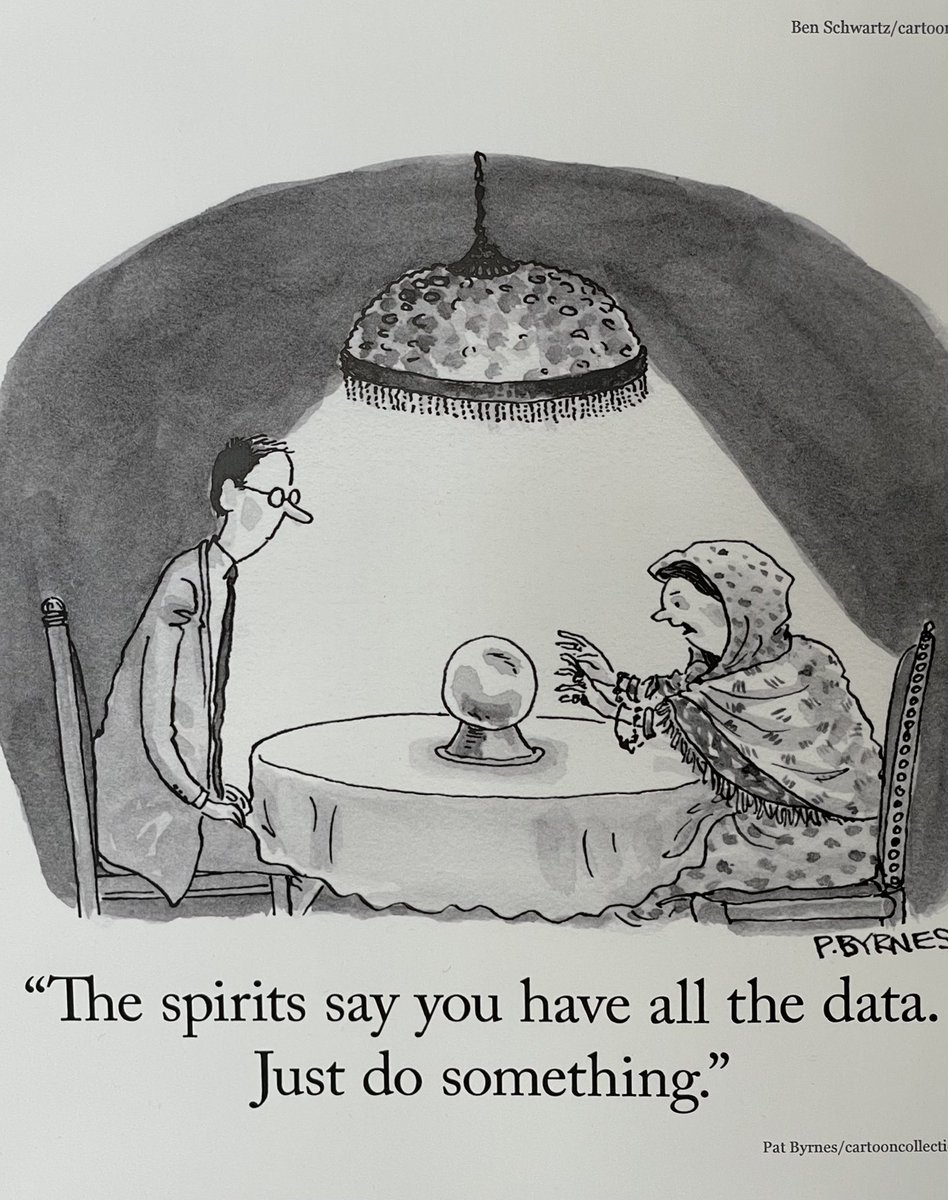
\includegraphics[width=0.7\textwidth,height=\textheight]{./part1/images/spirits.jpg}

}

\caption{Towards evidence-based decision making}

\end{figure}

\hypertarget{feedback}{%
\section*{Feedback}\label{feedback}}
\addcontentsline{toc}{section}{Feedback}

\markright{Feedback}

If you have any questions, wish to correct any technical or textual
mistakes, or wish to suggest improvements to this handbook, plese get in
touch with the Global CCCM Cluster Information Management Officers (IMO)
Brian Mc Donald -
\href{mailto:bmcdonald@iom.int}{\nolinkurl{bmcdonald@iom.int}} or Alisa
Ananbeh - \href{mailto:ananbeh@unhcr.org}{\nolinkurl{ananbeh@unhcr.org}}

\begin{quote}
We would like to thank everybody for their support in developing this
handbook and hope that you find it accessible and useful

\begin{itemize}
\tightlist
\item
  the CCCM Cluster team
\end{itemize}
\end{quote}

\hypertarget{acknowledgements}{%
\section*{Acknowledgements}\label{acknowledgements}}
\addcontentsline{toc}{section}{Acknowledgements}

\markright{Acknowledgements}

The content in this handbook are drawn from three main sources:

\begin{itemize}
\item
  The experience, advice and materials from our CCCM colleagues in the
  field.
\item
  Guidance materials developed at the global-level from inter-agency
  platforms including the Global Information Management Working Group
  and from other Clusters.
\item
  Many excellent information management trainings including: OCHA's
  \href{https://www.humanitarianresponse.info/en/operations/simulation-training/caim}{Coordinated
  Assessment and Information Management training (CAIM)}; and
  \href{https://www.acaps.org/humanitarian-analysis-programme-hap}{ACAPS's
  Humanitarian Analysis Program}.
\end{itemize}

\part{Humanitarian IM}

\hypertarget{data-literacy}{%
\chapter{Data Literacy}\label{data-literacy}}

\begin{tcolorbox}[enhanced jigsaw, colframe=quarto-callout-warning-color-frame, title=\textcolor{quarto-callout-warning-color}{\faExclamationTriangle}\hspace{0.5em}{Warning}, toptitle=1mm, toprule=.15mm, colbacktitle=quarto-callout-warning-color!10!white, breakable, arc=.35mm, coltitle=black, bottomrule=.15mm, titlerule=0mm, opacityback=0, rightrule=.15mm, bottomtitle=1mm, leftrule=.75mm, left=2mm, opacitybacktitle=0.6, colback=white]

This chapter is in draft stage.

\end{tcolorbox}

The purpose of this chapter is to introduce the reader to the concept of
data, what it is, how it used in humanitarian response and its relevance
in the role of information management. This chapter forms an important
basis for subsequent chapters as it aims to clearly describe key
concepts around data to ensure their clear and shared understanding.
This shared vocabulary is vital for the collaboration needed at the
various stages of the data's lifecycle. This chapter is primarily aimed
at IM's but is also relevant to any humanitarian involved to any degree
in evidence-based decision making.\footnote{From the
  \href{files/Reference\%20Module\%20for\%20Cluster\%20Coordination\%20at\%20Country\%20Level.pdf}{IASC
  Reference Module for Cluster Coordination at Country Level, revised
  July 2015}}

\begin{figure}

{\centering 
\includegraphics[width=0.7\textwidth,height=\textheight]{part1/./images/idontthinkitmeanswhatyouthinkitmeans.jpg}

}

\caption{A shared understanding of terms is important for engagement
around data}

\end{figure}

\hypertarget{what-is-data}{%
\section{What is data?}\label{what-is-data}}

Data is the physical representation of information in a manner suitable
for communication, interpretation, or processing by human beings or by
automatic means.\footnote{More details on
  \href{https://www.humanitarianresponse.info/en/programme-cycle/space}{HumanitarianResponse.info}}
It can be structured or unstructured, can come in many different forms
(human-readable or machine-readable) and can come from any number of
sources, using any number of methods. While the terms \emph{data},
\emph{information} and \emph{knowledge} are quite often used
interchangeably it is helpful to think of information as data integrated
into context, and knowledge as a collection of information, processed in
a way that provides learning.

\hypertarget{what-does-it-look-like}{%
\section{What does it look like?}\label{what-does-it-look-like}}

Data is all around us but is usually messy and unstructured. Processing
this information into a structure that can provide sense is at the core
of IM. This `sense-making' can use different approaches - an experienced
camp manager may decide to walk into a new camp, walk around it
observing it, deciding on what actions they need to prioritize. Another
may prefer to set up a list of indicators to measure specific needs in
the camp. The approaches are different (and quite often complimentary)
but the goal and process are to a large extent the same.

:::\{admonition\} Exercise Take a look at your desk and choose an
object. Describe the attributes of that item. Perhaps you can describe
the items colour, its length, its width, its texture, the materials its
constructed from or how effective it is for your work. A surprising
amount of data can be gathered from even the simplest of objects. :::

To get from messy data to structured that that can be used - by itself,
or more commonly in conjunction with other datasets - a degree of
organizing, tagging or categorizing must take place. If a survey is
used, those categories are determined by the questions asked the type of
questions and the response options. When setting these categories it is
very important that each person involved with the data - from the person
giving the response, the enumerator right up to those whose programmatic
decisions it informs - has a clear and common understanding of what and
how a concept is captured in these categories.

\hypertarget{formats}{%
\subsection{Formats}\label{formats}}

Valuable humanitarian data can often start out as paper survey
responses, hand written notes (ie. distribution details) or as
handwritten notes (such as from Focus Group Discussions). To aid the
cleaning, processing and management of this data, digitization may be
required. Digital data can be stored in a number of the following
formats and is closely linked to the tools used to gather and/or store
the data:

\begin{itemize}
\item
  \textbf{Tabular data:} By far the most common format for humanitarian
  data, Excel or Comma Separated Value (CSV) files show data as a table
  where each column represent as variable in your data and each row
  ideally represents an observation. \footnote{For a detailed
    explanation of RGB and CMYK and how they differ, see
    \href{https://en.99designs.ch/blog/tips/correct-file-formats-rgb-and-cmyk/}{here}}
\item
  \textbf{Relational databases:} Data cant always be represented in a
  single table. Quite often there is a need to present the data across
  multiple tables, showing the linkages(relationships) between variables
  in different table. Relational databases provide an underlying data
  model for most modern websites and software. An example use for a
  relational database could be in the recording of trainings, where one
  table contains rows, each representing a single training while a
  second table contains the list of participants. The relationships
  between these two tables could be defined as \emph{each training can
  contain multiple participants} and \emph{each participant can attend
  multiple trainings}
\item
  \textbf{APIs} To aid the access and transfer of data, it is very
  common for modern software systems to have an API, in which other
  websites (or data analysis tools) can request data from the underlying
  data store. The most common file format for these is called JSON, a
  semi-human readable format with the advantage over tabular formats in
  that is can represent messy semi-structured data or complex
  relationships that would otherwise require a database. \footnote{ACAPS
    have a great guide on the
    \href{https://www.acaps.org/use-colour-data-display}{Use of Colour
    in Data Display}}
\item
  \textbf{Spatial:} Spatial data formats such as .shp, .gpg, .geojson
  .geotiff or .dem are used to store 2d or 3d spatial data. Most of
  these formats can display or export to tabular formats.
\end{itemize}

\begin{figure*}

{\centering 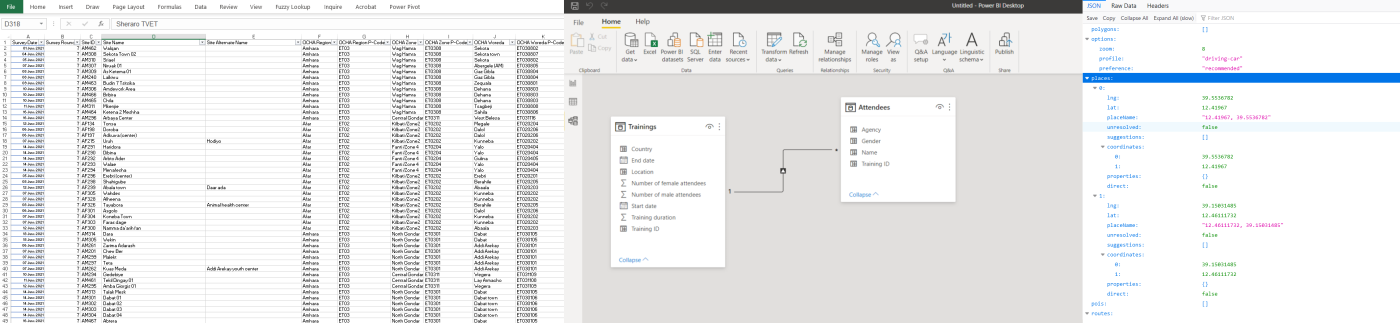
\includegraphics[width=0.7\textwidth,height=\textheight]{part1/./images/formats.png}

}

\caption{Examples of data as tables, a relational database, and as JSON
from an travel distance API}

\end{figure*}

\hypertarget{sources}{%
\subsection{Sources}\label{sources}}

\begin{itemize}
\tightlist
\item
  Common Operating Datasets (CODs)
\item
  HDX
\item
  Internal systems
\item
  Others
\item
  Non traditional sources
\end{itemize}

\hypertarget{data-concepts}{%
\section{Data concepts}\label{data-concepts}}

\hypertarget{values}{%
\subsection{Values}\label{values}}

Simple data values can be numeric; such as an integer (whole number) or
float; boolean, such as a yes/no or true/false; or a string, a sequence
of symbols such as a text answer. Compound values are combinations of
simple values. Examples include dates, time, or list of values (such as
a list of answers to a multiple choice question) \footnote{For a deeper
  dive into technical writing, this free
  \href{https://developers.google.com/tech-writing/overview}{Google
  course} is highly recommended}

\hypertarget{types-of-data}{%
\subsection{Types of data}\label{types-of-data}}

Variables (items of data) can spilt into two groups, quantitative
(numeric) or categoric (no inherent order). Quantitative variables can
either be discrete, meaning they have a finite number of values (eg
household size) or continuous, meaning an infinite number of values are
possible (eg. a persons height or distance to a health facility)

\hypertarget{scales}{%
\subsection{Scales}\label{scales}}

Data can be classified under the following 4 scales of measurement:

\begin{itemize}
\item
  \textbf{Nominal scales}: Nominal values/variables, sometimes called
  \emph{categorical values} don't have a numeric value so cannot be
  added, subtracted or multiplied. They do not have an order. For
  example, the name of a district that an IDP is from.
\item
  \textbf{Ordinal scale}: Contains values that can be put in order. For
  example, the levels of satisfaction with a training.
\item
  \textbf{Interval scale}: Contains ordinal numbers with meaningful
  divisions. For example, temperature or time.
\item
  \textbf{Ratio scale}: Ratio scales have all of the characteristics of
  interval scales as well as a true zero. For example, a persons height.
\end{itemize}

\begin{figure*}

{\centering 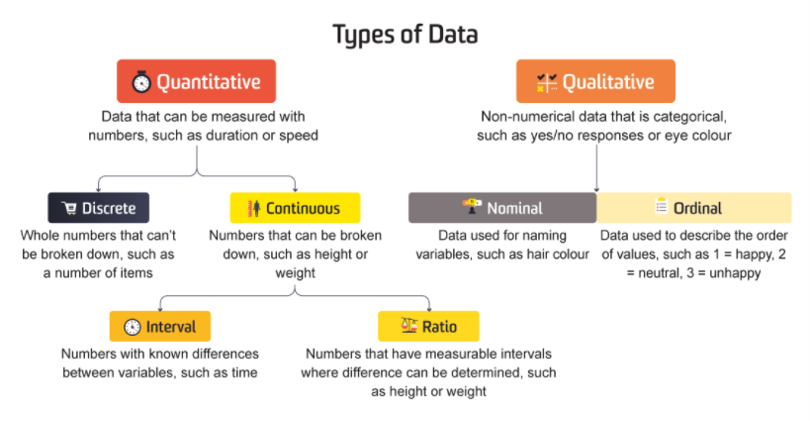
\includegraphics[width=0.7\textwidth,height=\textheight]{part1/./images/typesofdata.png}

}

\caption{Types of data and how they relate}

\end{figure*}

\hypertarget{goalstrategic-objective}{%
\subsection{Goal/Strategic Objective}\label{goalstrategic-objective}}

A specific end result desired or expected to occur as a consequence, at
least in part, of an intervention or activity. It is the higher order
objective that will assure national capacity building to which a
development intervention is intended to contribute.

\hypertarget{impact}{%
\subsection{Impact}\label{impact}}

Impact implies changes in people's lives. This might include changes in
knowledge, skill, behaviour, health or living conditions for children,
adults, families or communities. Such changes are positive or negative
longterm effects on identifiable population groups produced by a
development intervention, directly or indirectly, intended or
unintended.

\hypertarget{outcome}{%
\subsection{Outcome}\label{outcome}}

Outcomes represent changes in the institutional and behavioral
capacities for development conditions that occur between the completion
of outputs and the achievement of goals.

\hypertarget{outputs}{%
\subsection{Outputs}\label{outputs}}

Outputs are changes in skills or abilities and capacities of individuals
or institutions, or the availability of new products and services that
result from the completion of activities within a development
intervention within the control of the organization. They are achieved
with the resources provided and within the time period specified.

\hypertarget{activities}{%
\subsection{Activities}\label{activities}}

Actions taken or work performed through which inputs, such as funds,
technical assistance and other types of resources, are mobilized to
produce specific outputs.

\hypertarget{inputs}{%
\subsection{Inputs}\label{inputs}}

The financial, human, material, technological and information resources
used for development interventions.

\hypertarget{indicators}{%
\subsection{Indicators}\label{indicators}}

Usually separated into two categories: - Need indicators: a quantitative
or qualitative unit of measurement of need which when monitored
periodically can be used as a measure of impact. - Response/performance
indicators: used to measure outputs or outcomes.

\hypertarget{target}{%
\subsection{Target}\label{target}}

Specifies a particular value that an indicator should reach by to meet
agreed standard of service or programme goals. Setting target values for
most indicators requires a level of contextualization and can be
influences by external factors such as resources available.

\hypertarget{standard}{%
\subsection{Standard}\label{standard}}

\ldots{}

\hypertarget{benchmark}{%
\subsection{Benchmark}\label{benchmark}}

Reference point or standard, including norms, against which progress or
achievements can be assessed. A benchmark refers to the performance that
has been achieved in the recent past by other comparable organizations,
or what can be reasonably expected to have been achieved in similar
circumstances.

\hypertarget{primary-data-vs-secondary-data}{%
\subsection{Primary data vs secondary
data}\label{primary-data-vs-secondary-data}}

\ldots{}

\begin{center}\rule{0.5\linewidth}{0.5pt}\end{center}

\hypertarget{information-management-tips}{%
\section{Information Management
tips}\label{information-management-tips}}

The following tips are a collection of commonly encountered issues in
humanitarian IM and how to avoid them. The tips are a shortened from
their usual form to avoid overlap with other chapters where many of the
issues are expanded in more detail.\footnote{Adapted from The Chicago
  Guide to Writing about Numbers, by Jane E. Miller}

\hypertarget{use-excel-for-numerical-data}{%
\subsection{Use Excel for numerical
data}\label{use-excel-for-numerical-data}}

\begin{figure*}

{\centering 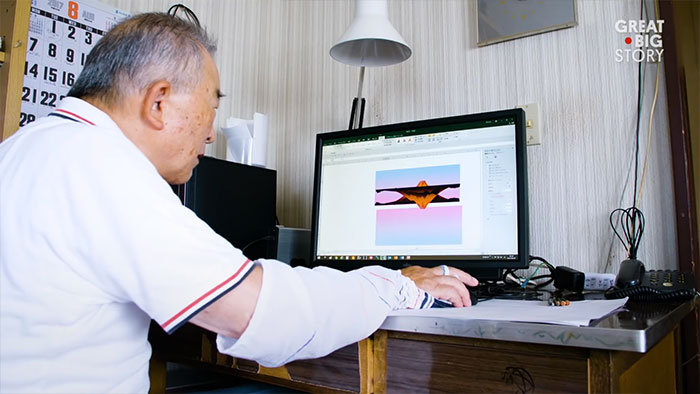
\includegraphics[width=0.7\textwidth,height=\textheight]{part1/./images/paintingwithexcel.jpg}

}

\caption{Tatsuo Horiuchi uses Excel to paint beautiful Japanese
lanscapes. Don't follow Tatsuo}

\end{figure*}

Don't use software such as Word for gathering and analysing numerical
data. Likewise, be careful not to use Excel to over visualise how your
data is represented. Simple, well structured data is best for analysis
and sharing with others.

\hypertarget{save-often-use-versioning-and-name-files-sensibly}{%
\subsection{Save often, use versioning, and name files
sensibly}\label{save-often-use-versioning-and-name-files-sensibly}}

\begin{figure*}

{\centering 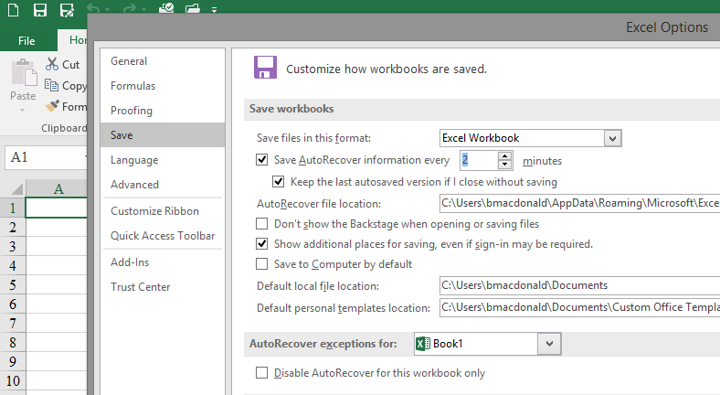
\includegraphics[width=0.7\textwidth,height=\textheight]{part1/./images/saveoften.png}

}

\caption{Click save!}

\end{figure*}

You don't want to work all day on an analysis to suddenly find that the
fil crashed before you had a chance to save it. In Excel, there is an
option to have your files autosave at a specified interval.

If saving to OneDrive or Sharepoint, you will see a small downward arrow
which allows youto view the file's \emph{Version History}. to view or
roll back to previous version of a document. Alternatively you can save
multiple versions of the file following certain milestones or use a
software versioning software such as Git.

Try have you and your team use a consistent, welll understood naming
convention for files. The format I use is as follows:
\emph{{[}year{]}{[}month(2digists){]}{[}date{]}-{[}initials{]}-{[}version{]}}.
For example 20182307-IMtips-BMD-v1.xlsx \emph{File} \textgreater{}
\emph{Options} to get Excel to save more regularly

\hypertarget{backup-your-data}{%
\subsection{Backup your data}\label{backup-your-data}}

What if your computer crashes or is stolen?\\
What if you need to collaborate on a file?\\
Make use of Onedrive/Sharepoint. Onedrive is ideal for working documents
(you can right-click on a file and share it collaboratively).

\hypertarget{check-for-existing-data-communicate}{%
\subsection{Check for existing data,
communicate}\label{check-for-existing-data-communicate}}

Networking and communication are important but sometimes overlooked
skills for IM. It's important to know what other agencies and clusters
are planning in terms of data collection and what challenges they are
facing that may be better addressed with a collective approach. Checking
for pre-existing data or planning assessments can help avoid duplication
of efforts and unnecessarily \emph{reinventing the wheel}.

\hypertarget{use-mobile-data-collection}{%
\subsection{Use mobile data
collection}\label{use-mobile-data-collection}}

The use of mobile data collection tools such as
\href{https://kobo.humanitarianresponse.info/}{Kobo Toolbox} support
faster and more robust data collection. By enforcing checks on data
inputs it reduces input errors, while also removing time consuming and
error-prone tasks of manual data entry of paper forms.

While ideal for surveys/assessments, be careful not to over-fit such
tools into scenarios that require \emph{case management} type
functionality.

\hypertarget{consistent-variable-naming}{%
\subsection{Consistent variable
naming}\label{consistent-variable-naming}}

\emph{Are we talking about the same thing?} The terms/concepts describe
in your surveys and data - does everyone have a clear and shared
understanding of what they mean? Are you reusing well known and tested
terms or are you inventing new ones. \footnote{Data journalism put
  increasing emphasis on the need for a good annotation layer, as can be
  seen by this article from the
  \href{https://www.ft.com/content/4743ce96-e4bf-11e7-97e2-916d4fbac0da}{Financial
  Times}}

\hypertarget{understand-meta-data}{%
\subsection{Understand meta-data}\label{understand-meta-data}}

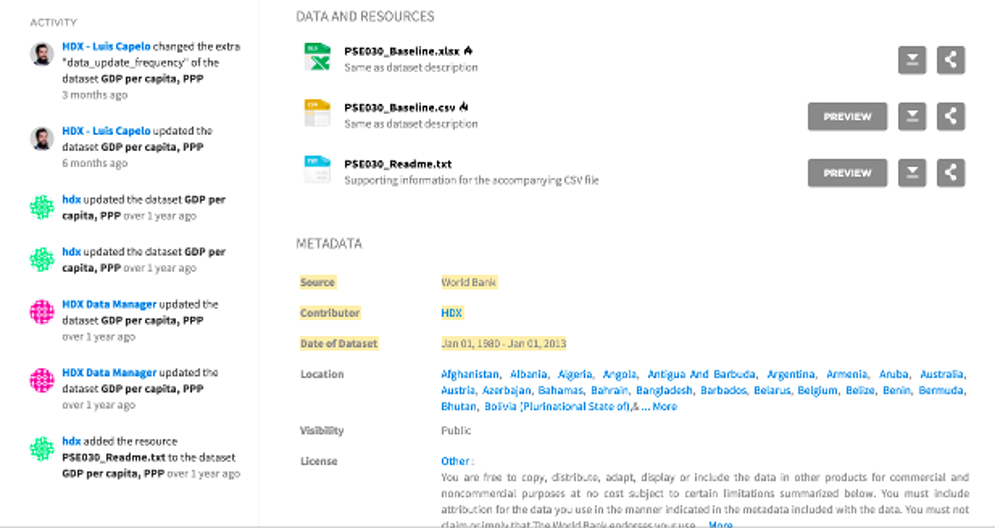
\includegraphics{part1/./images/metadata.png}\\
\ldots and why it is important. Meta-data is data that described data.
For example, your survey data files should contain information
describing where the data was collected, on which dates, the methodology
used and relevant focal point. Including metadata in your datasets is an
important habit for IMs, as it encourages reuse of the data and
signifies a robust approach to analysis.

\hypertarget{spreadsheets---only-one-piece-of-information-per-cell}{%
\subsection{Spreadsheets - only one piece of information per
cell}\label{spreadsheets---only-one-piece-of-information-per-cell}}

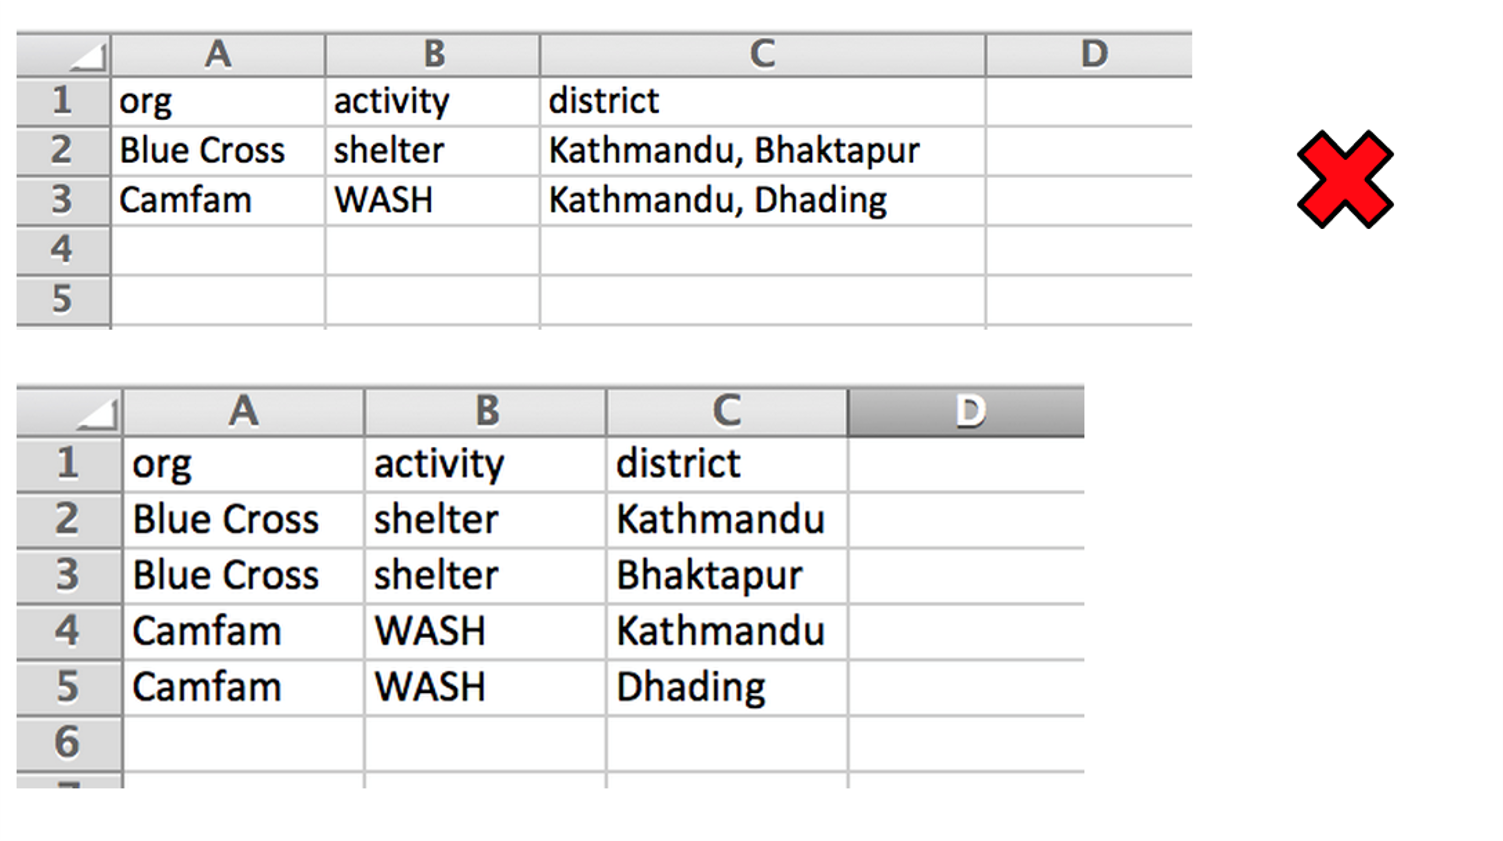
\includegraphics{part1/./images/onepercell.png}\\
Storing multiple points of data in a single cell makes many types of
analysis very difficult. Where possible try to expand these values onto
their own rows (sometimes called ``exploding'' or ``melting''.)

\hypertarget{record-data-at-a-granular-level-and-aggregate-up}{%
\subsection{Record data at a granular level and aggregate
up}\label{record-data-at-a-granular-level-and-aggregate-up}}

When you have data at a low unit of measurement, for example, the number
of people using a specific Complaints and Feedback (CFM) desk, it is
straightforward to aggregate that data to a higher unit, for example,
the number of people using CFMs in a district. However, be careful of
receiving data already aggregated as it is usually not possible to
disaggregate it into its component parts. If your analysis depends on
having data at a certain unit-level, make sure to have it collected or
sent to you in at least the same or lower level of disaggregation.
Aggregation may hide or disregard useful data useful for your analysis
or quality control.

\hypertarget{learn-pivot-tables}{%
\subsection{Learn pivot tables}\label{learn-pivot-tables}}

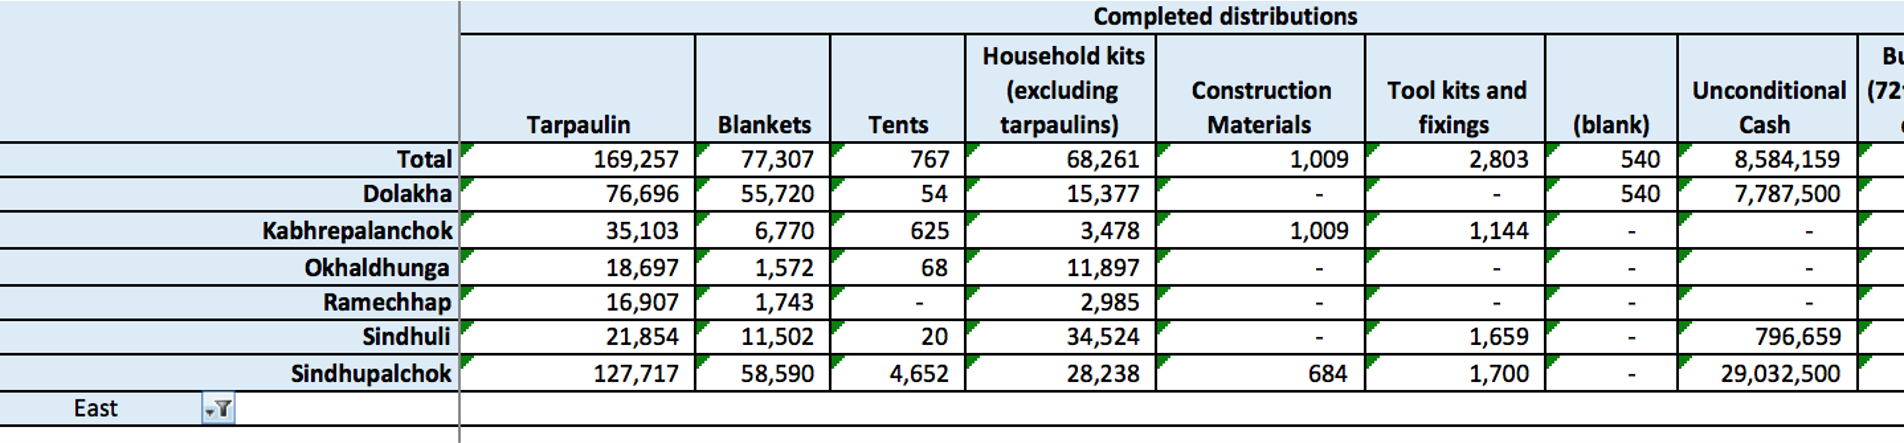
\includegraphics{part1/./images/pivot.png} Pivot tables are a powerful
tool for aggregating data in Excel. (also called ``groupby'' in other
software)

\hypertarget{learn-vlookup-and-index-match}{%
\subsection{Learn VLOOKUP and Index
Match}\label{learn-vlookup-and-index-match}}

\begin{figure}

{\centering 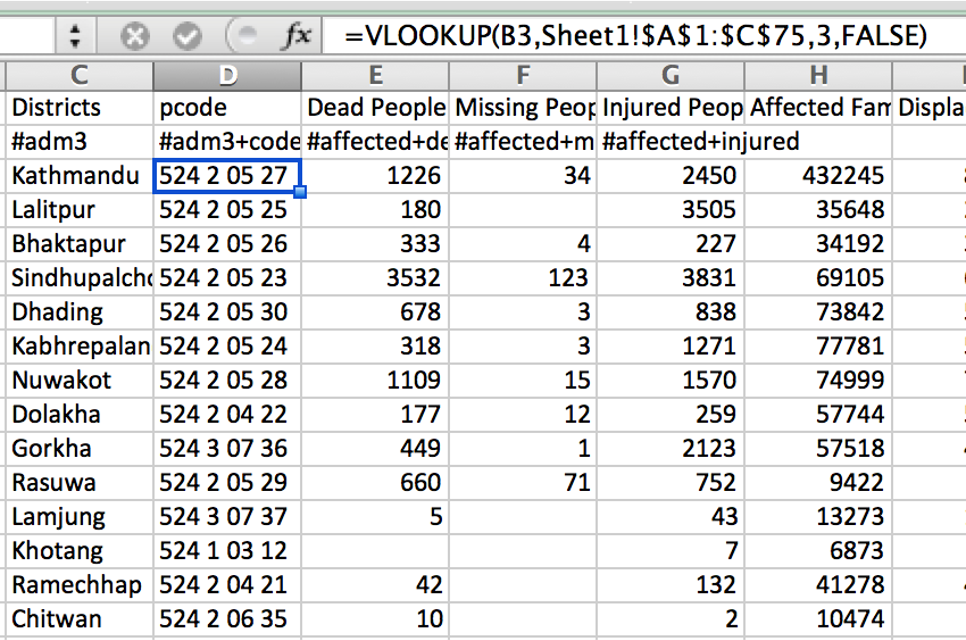
\includegraphics{part1/./images/vlookup.png}

}

\caption{vlookup}

\end{figure}

\hypertarget{dont-merge-cells-in-a-spreadsheet}{%
\subsection{Don't merge cells in a
spreadsheet}\label{dont-merge-cells-in-a-spreadsheet}}

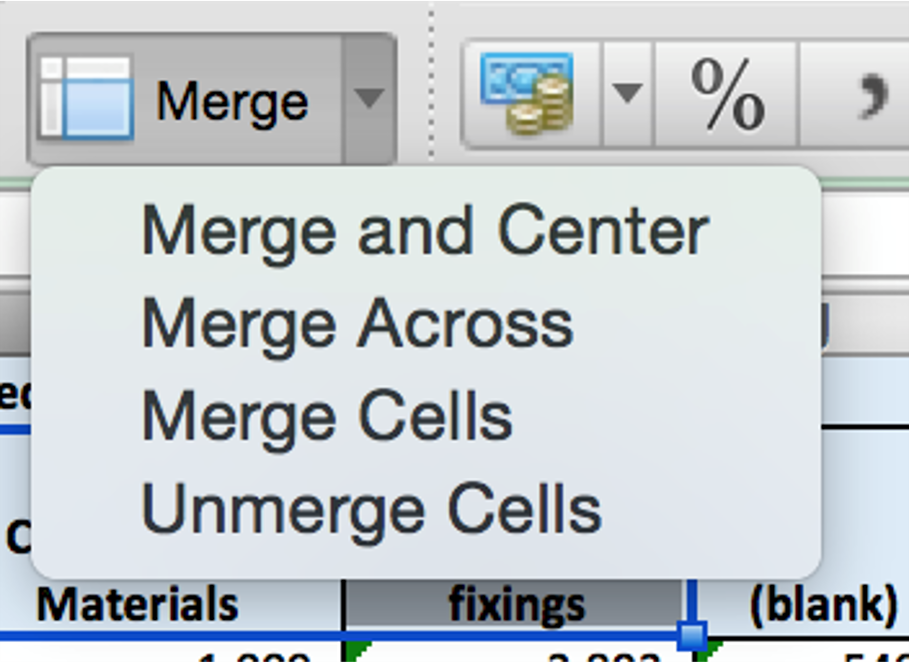
\includegraphics{part1/./images/merge.png}\\
Don't merge cells in a spreadsheet. Tables should contain an equal
number of rows and columns. Merging cells breaks pivoting and filtering
and goes against rule number 1 (when done for reasons of aesthetics).

\hypertarget{keep-data-types-and-names-consistent-in-columns}{%
\subsection{Keep data types and names consistent in
columns}\label{keep-data-types-and-names-consistent-in-columns}}

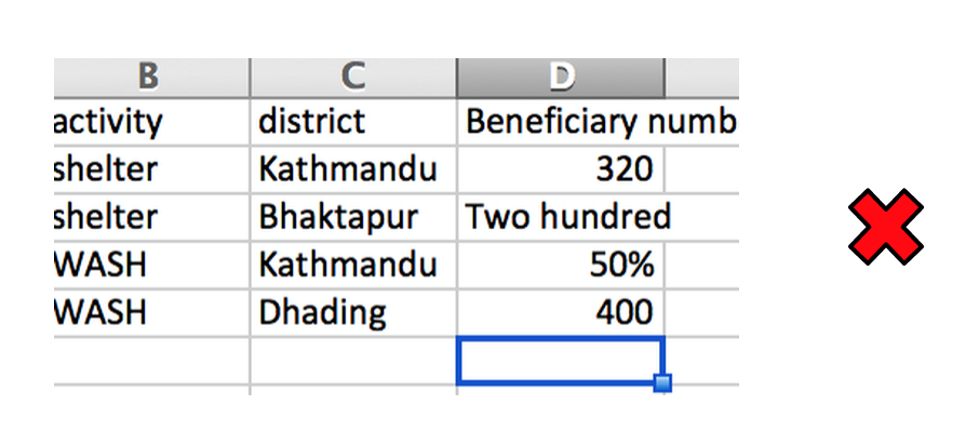
\includegraphics{part1/./images/names.png}\\
Make sure that the spelling (including case) and format of values remain
consistent for all values in a column.

\hypertarget{keep-all-similar-data-in-one-sheet}{%
\subsection{Keep all similar data in one
sheet}\label{keep-all-similar-data-in-one-sheet}}

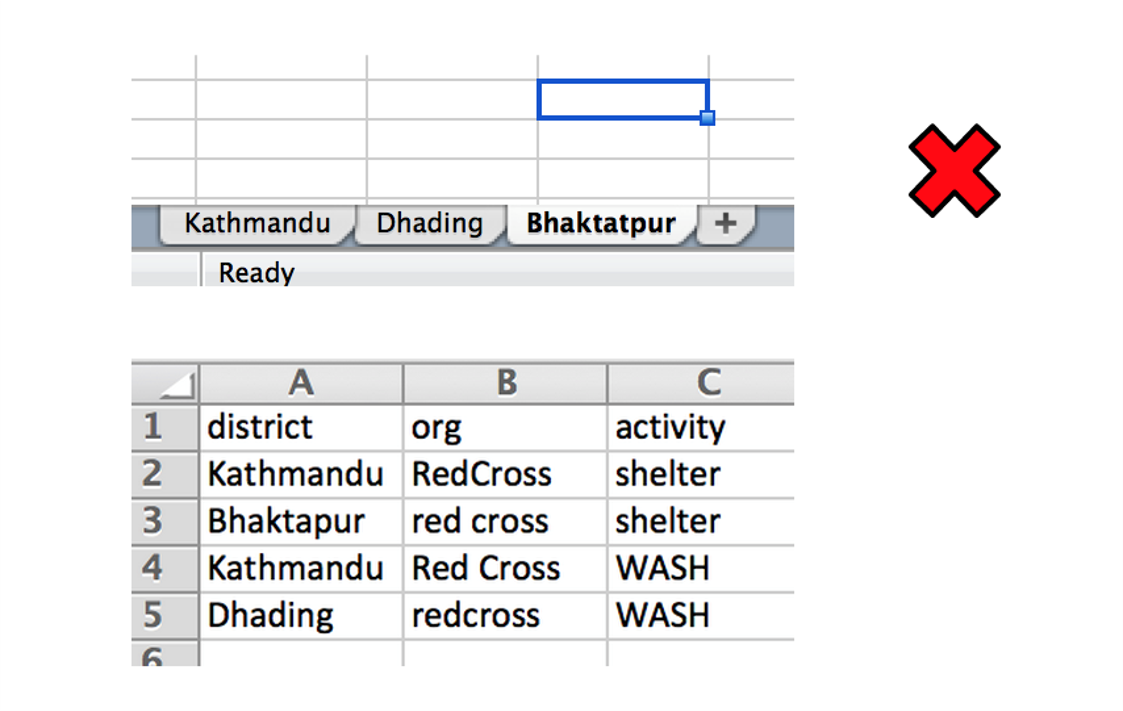
\includegraphics{part1/./images/1sheet.png}\\
Resist the temptation to split large datasets across tabs, using a tab
for each region etc. This makes analysis and consolidated storage and
management of the data harder. Instead add a column to capture the
category names.

\hypertarget{check-data-relationships}{%
\subsection{Check data relationships}\label{check-data-relationships}}

\begin{figure}

{\centering 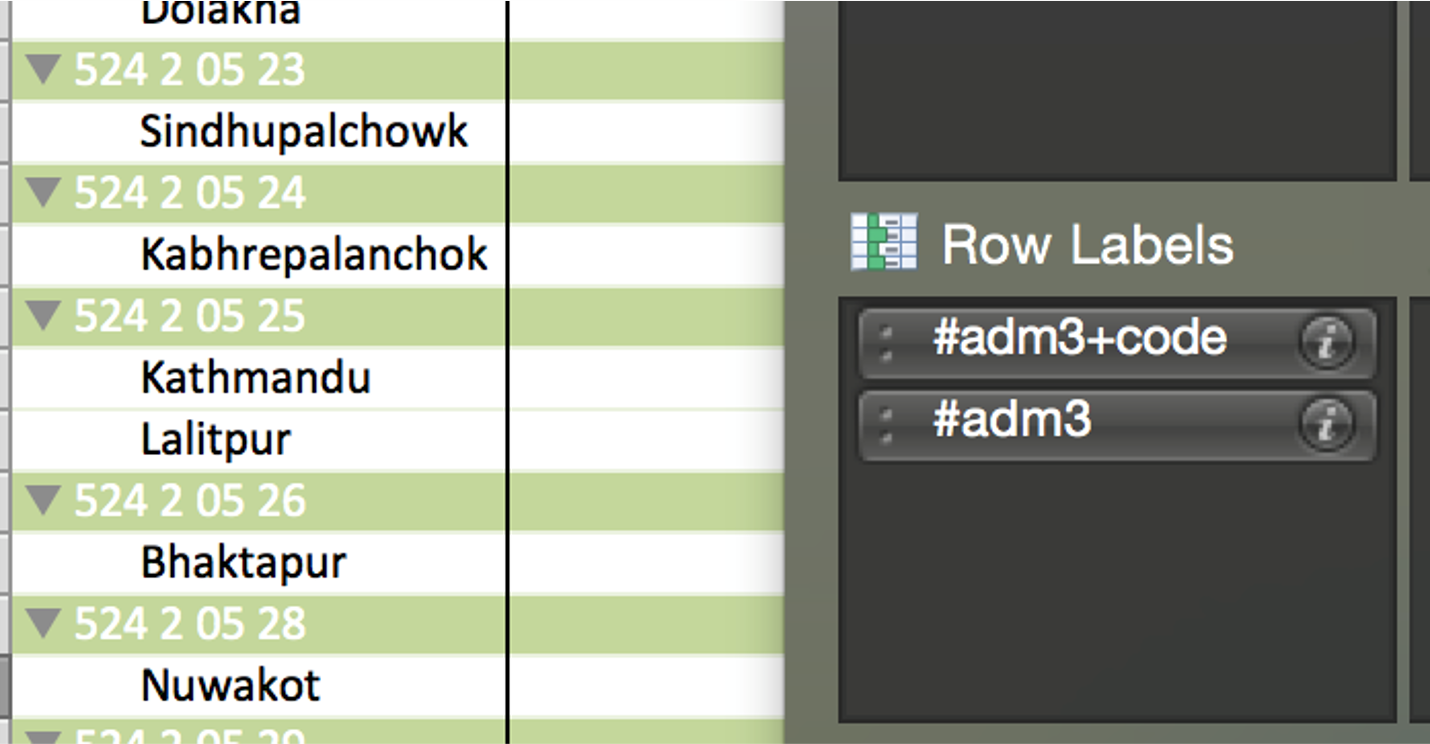
\includegraphics{part1/./images/checkrelationships.png}

}

\caption{check relationaships}

\end{figure}

\hypertarget{get-coordinates-for-point-data}{%
\subsection{Get coordinates for point
data}\label{get-coordinates-for-point-data}}

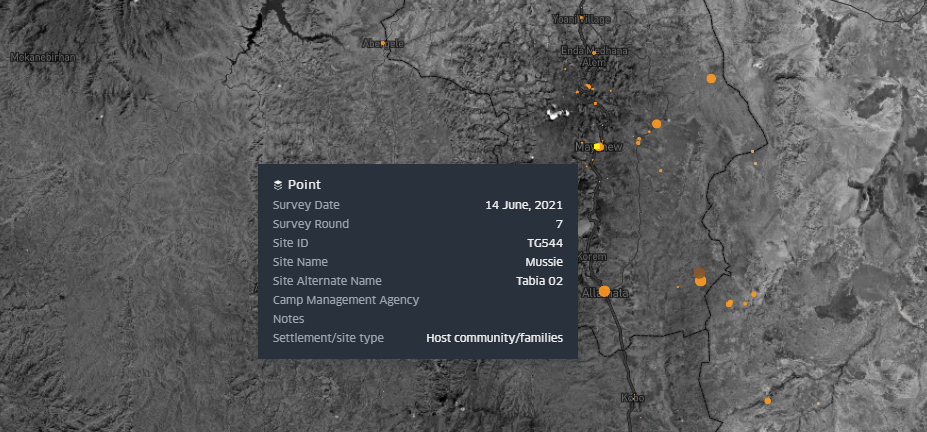
\includegraphics{part1/./images/pointdata.png}\\
If you have data that represents a point such as a hospital or a camp,
instead of just naming it or giving its address you could also collect
coordinates for it. There are many possible ways of doing this:

\begin{itemize}
\item
  Using any app on your phone that records GPS
\item
  In a mobile data collection tool such as Kobo Toolbox
\item
  Using a geocoder, which outputs coordinates for given addresses or
  locations. \href{http://nominatim.openstreetmap.org/}{Nominatim} is a
  free service using Open Street Map data.
\item
  The low tech approach of drawing on paper maps, digitizing later.
  \href{is\%20a\%20good\%20tool\%20for\%20this}{Fieldpapers}
\end{itemize}

\hypertarget{what-is-information-management}{%
\chapter{What is Information
Management?}\label{what-is-information-management}}

\begin{tcolorbox}[enhanced jigsaw, colframe=quarto-callout-warning-color-frame, title=\textcolor{quarto-callout-warning-color}{\faExclamationTriangle}\hspace{0.5em}{Warning}, toptitle=1mm, toprule=.15mm, colbacktitle=quarto-callout-warning-color!10!white, breakable, arc=.35mm, coltitle=black, bottomrule=.15mm, titlerule=0mm, opacityback=0, rightrule=.15mm, bottomtitle=1mm, leftrule=.75mm, left=2mm, opacitybacktitle=0.6, colback=white]

This chapter is in draft stage.

\end{tcolorbox}

..

\hypertarget{profiles}{%
\section{Profiles}\label{profiles}}

..

\hypertarget{skills-and-attitudes}{%
\section{Skills and attitudes}\label{skills-and-attitudes}}

.

\begin{figure}

{\centering 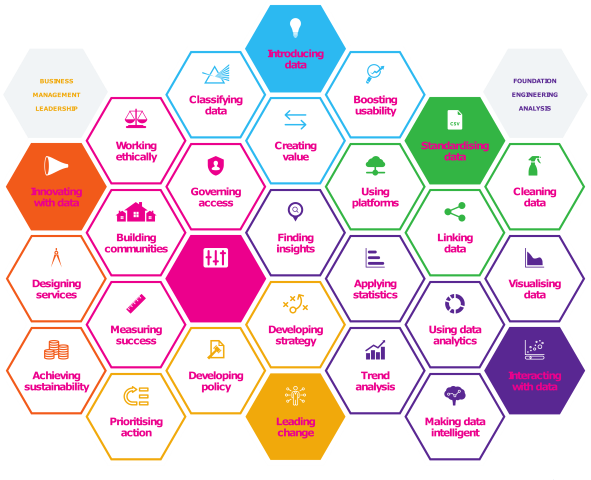
\includegraphics{part1/./images/dataskillsframework.png}

}

\caption{A Data Skills Framework by the
\href{https://theodi.org/article/data-skills-framework/}{ODI}}

\end{figure}

\hypertarget{responsibilities}{%
\section{Responsibilities}\label{responsibilities}}

\begin{itemize}
\tightlist
\item
  The core cluster functions and how they relate to IM.
\end{itemize}

\hypertarget{im-workflow}{%
\section{IM workflow}\label{im-workflow}}

.

\hypertarget{collection}{%
\subsection{Collection}\label{collection}}

This section discusses: - Secondary data review - Primary data
collection

\hypertarget{processing}{%
\subsection{Processing}\label{processing}}

.

\hypertarget{analysis}{%
\subsection{Analysis}\label{analysis}}

.

\hypertarget{dissemination}{%
\subsection{Dissemination}\label{dissemination}}

.

\hypertarget{design-acquire}{%
\chapter{Design \& Acquire}\label{design-acquire}}

This chapter is in draft stage.

Any information that doesn't not inform or change an decision is
worthless.

-- Sam L. Savage

\begin{itemize}
\tightlist
\item
  many illustrations start with ``data collection'' but this should not
  be the first step
\item
  secondary data review vs primary data
\item
  formulating the questions that need answering.
\item
  create a data analysis plan
\item
  common data sources
\item
  CODs
\item
  methods - KI. FGD
\item
  sampling
\item
  minimal viable information
\end{itemize}

\hypertarget{before-you-start-collecting-data.}{%
\section{Before you start collecting
data.}\label{before-you-start-collecting-data.}}

.stop and think. IM guidances sometimes present IM task in a linear
fashion that starts with \emph{data collection}. This is problematic.
Good analysis requires us to first start with an articulation of what
are the overarching questions that need answering and what decisions
will be informed by this evidence.

The next step is to take stock of existing data and to develop an
analysis plan linking your information needs to you existing data and/or
any potential future data collection exercises.

Collection of data has costs - it costs time, it has HR costs, it has
financial costs. It is important to understand these costs and viewing
them in relation to the value it provides to your decision making.
Similarly, when developing surveys, adding questions are no without
cost, as for each question that is added, there is a cognitive cost(more
questions = higher likelihood of mistakes), a time cost (longer surveys
take longer to do) and a quality cost (cleaning and data checks are more
difficult on larger datasets). Understand that 80\% of the value of your
survey will come from 20\% of your survey. As you add additional
questions to your survey, the value they add to your decision-making
diminishes. \footnote{From the
  \href{files/Reference\%20Module\%20for\%20Cluster\%20Coordination\%20at\%20Country\%20Level.pdf}{IASC
  Reference Module for Cluster Coordination at Country Level, revised
  July 2015}}

\begin{figure*}

{\centering 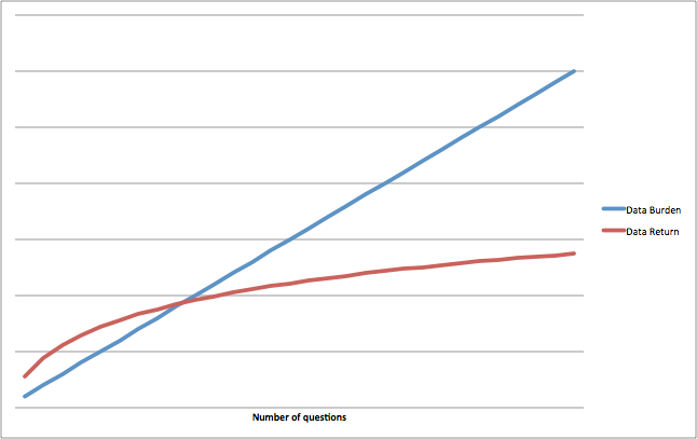
\includegraphics[width=0.7\textwidth,height=\textheight]{part1/./images/minimalviableinformation.png}

}

\caption{As your number of survey questions increase, the return on
effort gradually diminishes.}

\end{figure*}

\hypertarget{methodologies}{%
\section{Methodologies}\label{methodologies}}

\begin{itemize}
\tightlist
\item
  KI
\item
  FGD
\item
  Observations
\item
  Non traditional sources
\item
  Representativeness
\end{itemize}

\hypertarget{sampling}{%
\subsection{Sampling}\label{sampling}}

.

\hypertarget{analysis-1}{%
\chapter{Analysis}\label{analysis-1}}

This chapter is in draft stage.

.

\hypertarget{the-analysis-spectrum}{%
\section{The Analysis Spectrum}\label{the-analysis-spectrum}}

.
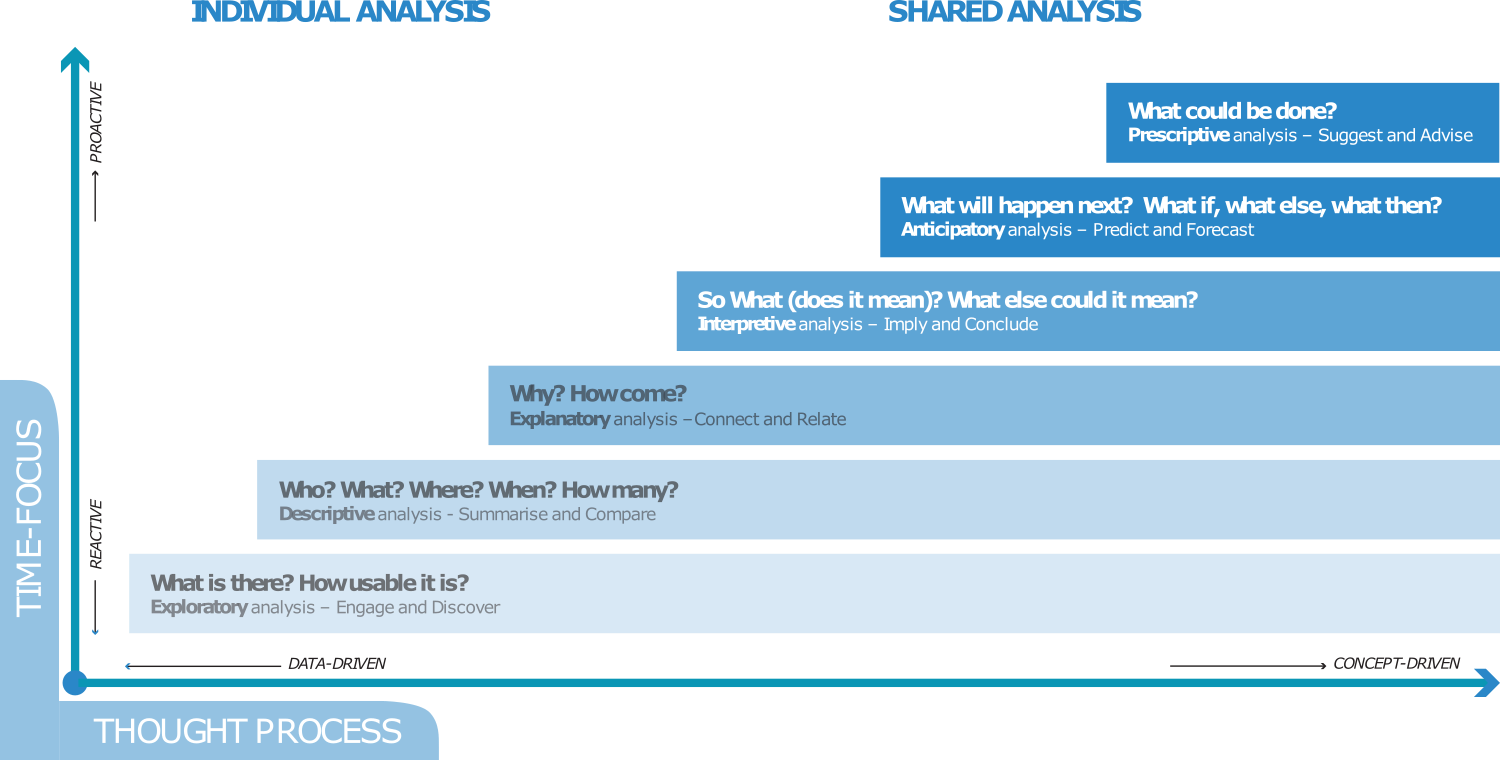
\includegraphics[width=0.7\textwidth,height=\textheight]{part1/./images/analysisspectrum.png}

\hypertarget{understanding-bias}{%
\section{Understanding Bias}\label{understanding-bias}}

.

\begin{figure*}

{\centering 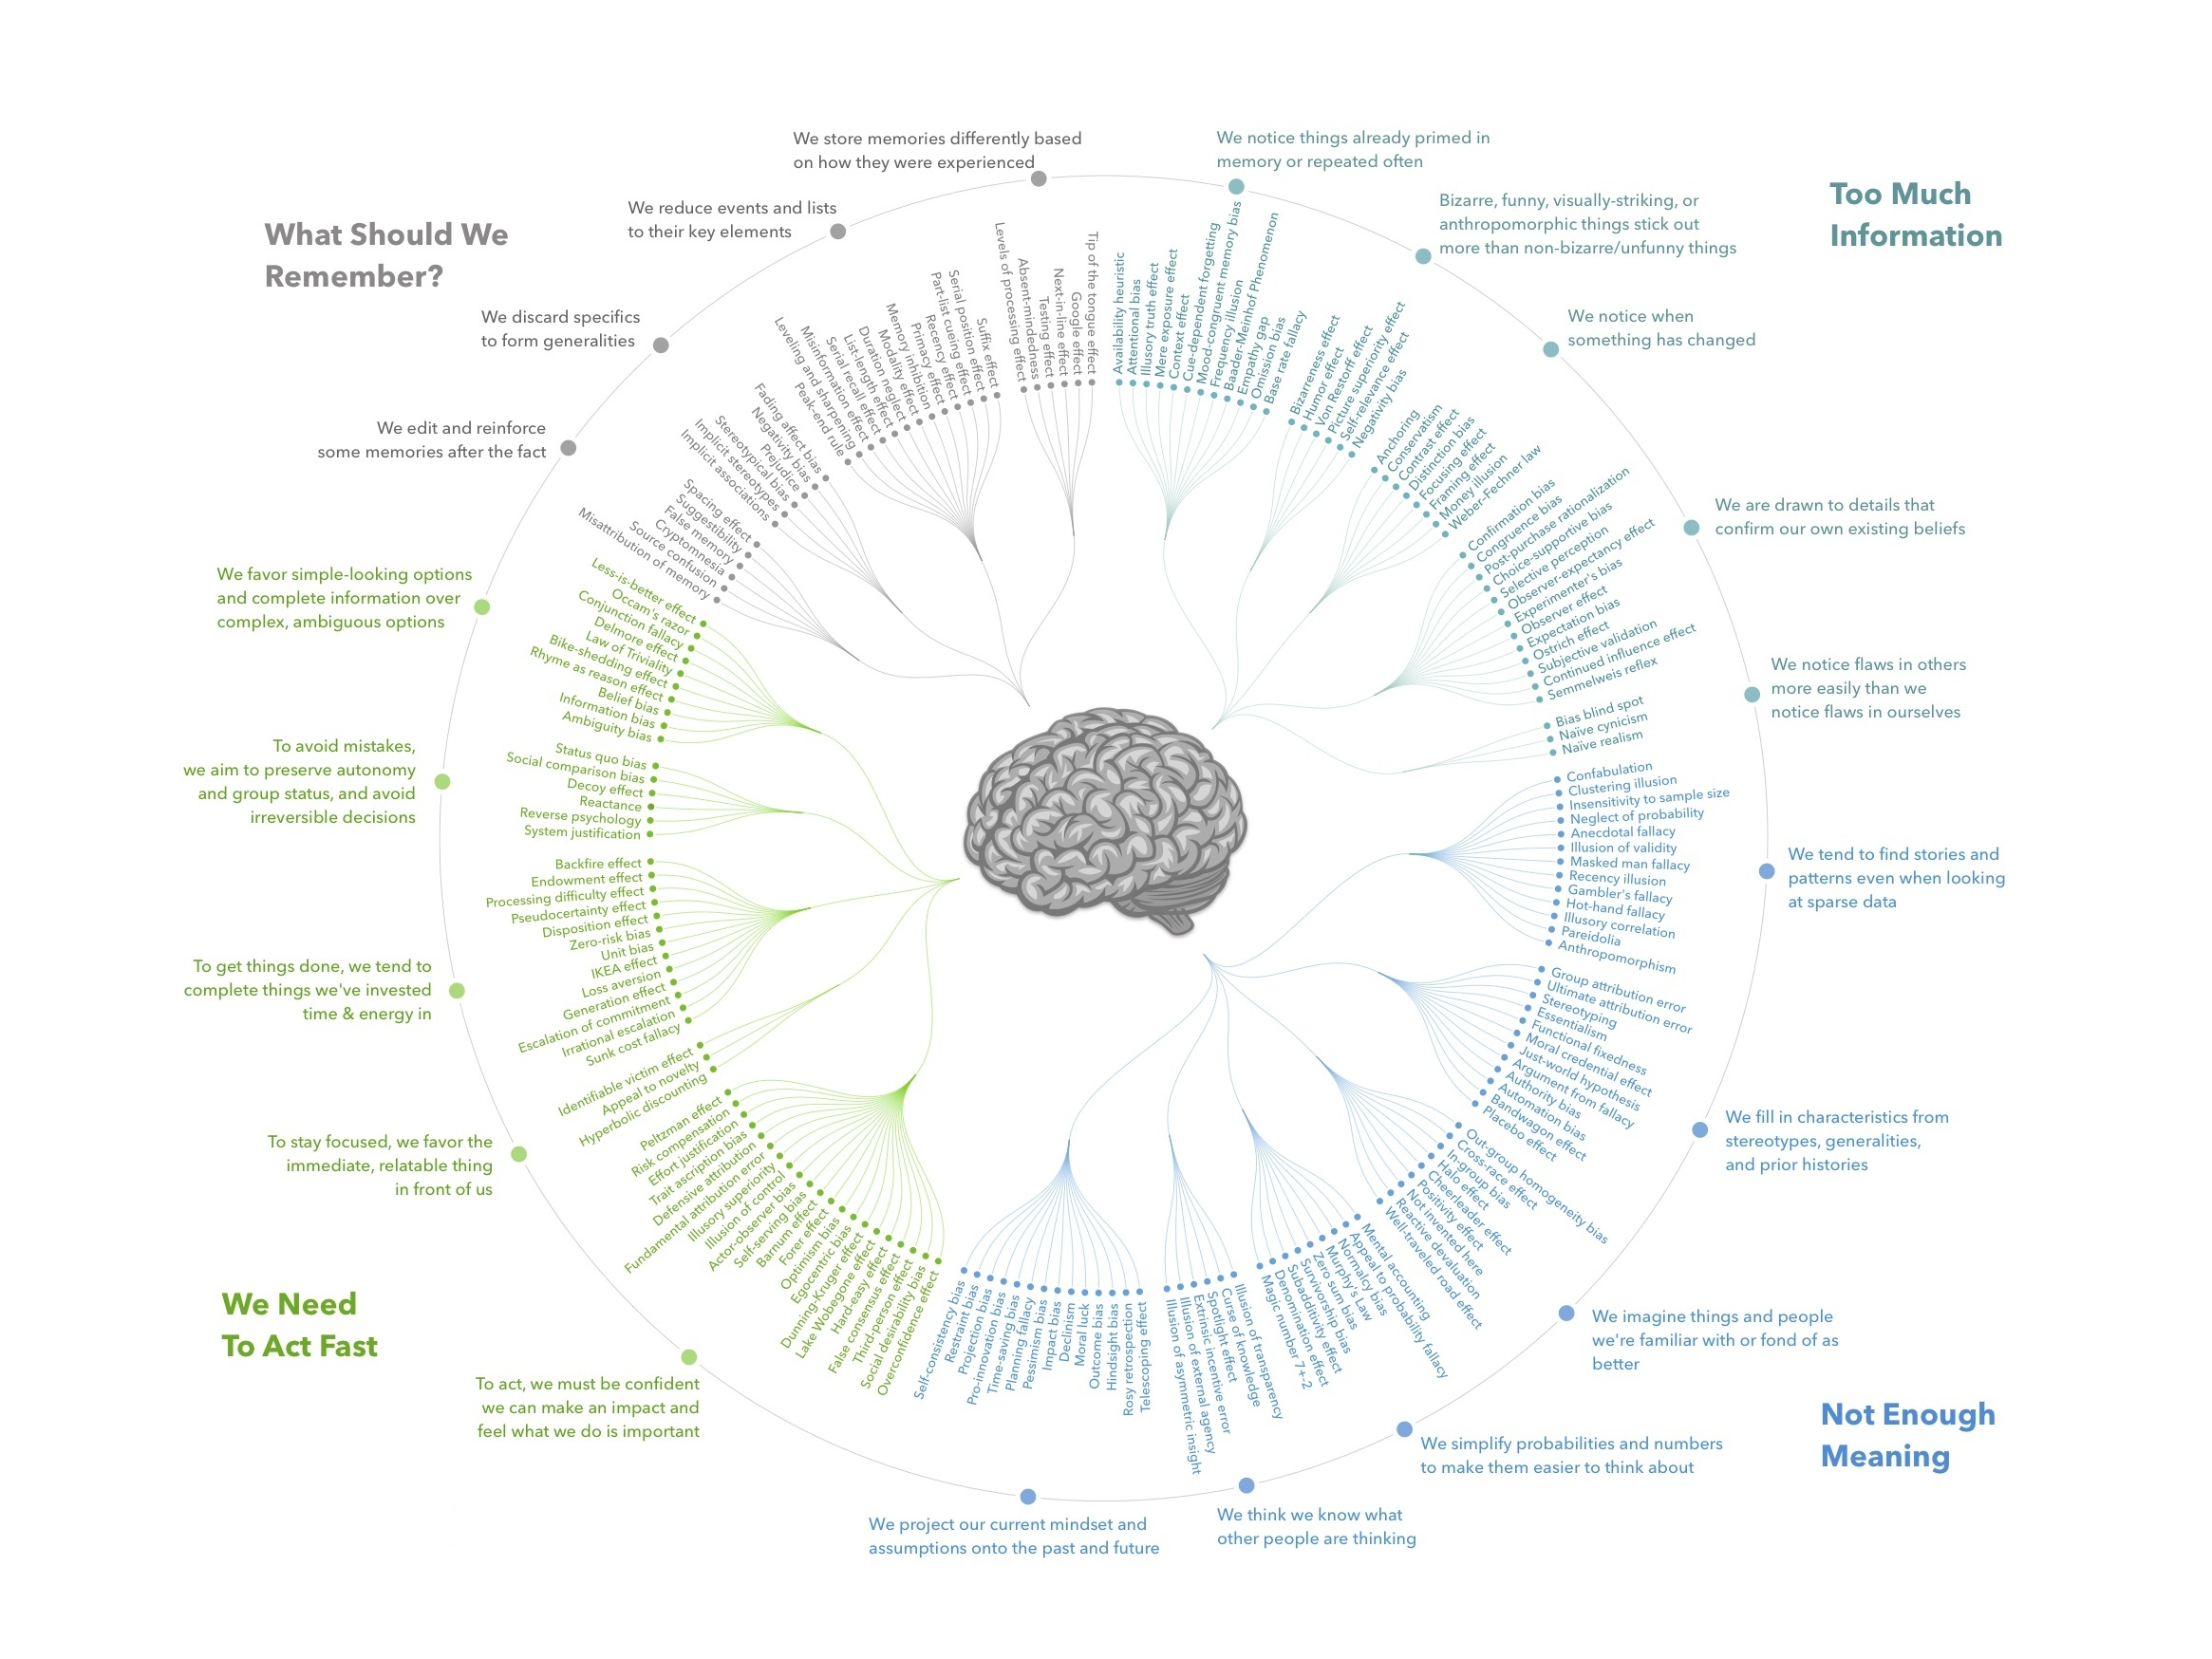
\includegraphics[width=0.7\textwidth,height=\textheight]{part1/./images/cognitive-bias.jpg}

}

\caption{188 Cognitive biases (adapted from Mangoongian 2021) -
\href{./images/cognitive-bias.jpg}{view larger}}

\end{figure*}

\hypertarget{communication-visualization}{%
\chapter{Communication \&
Visualization}\label{communication-visualization}}

Communication may be the final step in the IMs workflow but is by no
means the least important. The best analysis, using the best data
collection methods and tools are worthless if the communication of these
findings are insufficient to inform decisions. \footnote{For a deeper
  dive into technical writing, this free
  \href{https://developers.google.com/tech-writing/overview}{Google
  course} is highly recommended}

\hypertarget{how-to-write-about-numbers}{%
\section{How to write about numbers}\label{how-to-write-about-numbers}}

When preparing to write up an analysis, it is important to first
consider the following:

\textbf{Determine your objectives.} Is the intention to inform or update
a group on recent activities? Is it to provide insight on a particular
topic? Is it to change peoples understanding or decisions on an
particular operational issue? Is it to engage with people to gather
feedback or to take action?

\textbf{Identify your target audience.} What group or groups are you
targeting with the above objectives? You will need to tailor the
language(non technical experts may not be familiar with technical
language), length (shorter messages may be more suitable for general
public consumption) and style (different audiences have different lenses
in which they will consume and interpret your message).

There are seven basic principles about writing about numbers:
\footnote{Adapted from The Chicago Guide to Writing about Numbers, by
  Jane E. Miller}

\begin{enumerate}
\def\labelenumi{\arabic{enumi}.}
\item
  \textbf{Establish the context for your facts.} Your text should convey
  the ``who, what, when and where'' in which to ground your facts. Don't
  just assume that the audience has the same contextual understanding.
\item
  \textbf{Pick simple, plausible examples.} Using examples are a good
  way to transform abstract numbers to more tangible and relatable to
  the audiences experiences or understanding. An example of this could
  be used when describing density of the population of Rohingya refugees
  in Cox's Bazar, Bangladesh, where comparing the population number and
  area of the camp can be compared to that of a comparison city familiar
  to the audience.
\item
  \textbf{Select the right tools and media for the job.} The three basic
  tools for presenting quantitative information: prose, tables and
  charts. Choosing the most appropriate tool (or mix of them) and
  understanding their strengths and weaknesses, is important. Equally
  important is to use the most appropriate mix of media. Eg. Reports,
  interactive dashboards, infographics, video, social media, events.
\item
  \textbf{Defining your terms (and be careful with jargon).} Unnecessary
  use of of acronyms and jargon will likely exclude parts of your
  audience or cause misunderstanding due to unshared understanding of
  concepts. If acronyms must be used, it is good practice to show them
  alongside their long form at the point where they first appear.
\item
  \textbf{Reporting and interpreting.} Describing the numbers around an
  issue should be support by an explanation of ``what does that mean''
  that explains why that number is important or relevant.
\item
  \textbf{Specify magnitude and direction of an association.} Don't just
  say ``there are more displaced people in camp A than in camp B'',
  provide a number quantifying \emph{how} different it is. When
  explaining the relationship between variables it is also important to
  be clear on the direction of that relationship. For example ``IDPs in
  Camp A had a lower number of food complaints compared to the previous
  month''.
\item
  \textbf{Summarize patterns.} Rather than presenting a big table or
  graph showing the data and letting the viewer figure things out for
  themselves it is good to summarize and highlight patterns that
  contribute to the analysis and message.
\end{enumerate}

\begin{tcolorbox}[enhanced jigsaw, colframe=quarto-callout-tip-color-frame, title=\textcolor{quarto-callout-tip-color}{\faLightbulb}\hspace{0.5em}{Tip}, toptitle=1mm, toprule=.15mm, colbacktitle=quarto-callout-tip-color!10!white, breakable, arc=.35mm, coltitle=black, bottomrule=.15mm, titlerule=0mm, opacityback=0, rightrule=.15mm, bottomtitle=1mm, leftrule=.75mm, left=2mm, opacitybacktitle=0.6, colback=white]

\begin{itemize}
\tightlist
\item
  Tell a story
\item
  Choose hooks for your audience
\item
  Say it visually
\item
  Be transparent with the limitations of your analysis
\end{itemize}

\end{tcolorbox}

\hypertarget{data-visualization}{%
\section{Data Visualization}\label{data-visualization}}

Communicating with visuals can an effective way to communicate a
message, either on its own or alongside accompanying text. Good visuals
can help engaging the audience and quite often are a good way to convey
complex information in a simpler form.

\hypertarget{choosing-the-right-charts}{%
\subsection{Choosing the right charts}\label{choosing-the-right-charts}}

When visualising your data, the choice of chart depends on the quantity
and type of data you want to represent; the relationships in that data,
and ultimately, whether or not the graph clearly communicates your
message.\footnote{From the
  \href{files/Reference\%20Module\%20for\%20Cluster\%20Coordination\%20at\%20Country\%20Level.pdf}{IASC
  Reference Module for Cluster Coordination at Country Level, revised
  July 2015}}

The following is pseudo-decision tree, to support choosing the most
appropriate chart type depending on your data and it relationships.

\hypertarget{deviation}{%
\subsubsection{Deviation}\label{deviation}}

Emphasize variations (+/-) from a fixed reference point. Typically the
reference point is zero but it can also be a target or a long-term
average. Can also be used to show sentiment (positive/neutral/negative).

\textbf{Examples:} Showing the number of people entering or exiting a
site over a period of time. Showing satisfaction with a component in a
training. Demographics pyramid in a site, showing population breakdown
by age and gender.


\includegraphics{part1/images/deviation1.png}\\
\textbf{Diverging bar:} A simple standard bar chart that can handle both
negative and positive magnitude values.

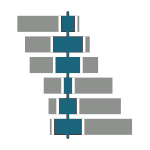
\includegraphics{part1/images/deviation2.png}\\
\textbf{Diverging bar:} Perfect for presenting survey results which
involve sentiment (eg disagree/neutral/agree).


\includegraphics{part1/images/deviation3.png}\\
\textbf{Spine:} Splits a single value into two contrasting components
(eg male/female).


\includegraphics{part1/images/deviation4.png}\\
\textbf{Surplus/deficit filled line:} The shaded area of these charts
allows a balance to be shown -- either against a baseline or between two
series.

\hypertarget{correlation}{%
\subsubsection{Correlation}\label{correlation}}

Show the relationship between two or more variables. Be mindful that,
unless you tell them otherwise, many readers will assume the
relationships you show them to be causal (i.e.~one causes the other).

\textbf{Examples:} Showing the relationships between areas of origin and
current location of displacement.

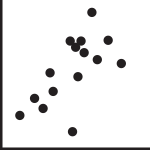
\includegraphics{part1/images/corellation1.png}\\
\textbf{Scatterplot:} The standard way to show the relationship between
two continuous variables, each of which has its own axis.

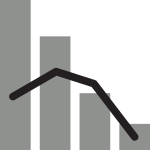
\includegraphics{part1/images/corellation2.png}\\
\textbf{Column + line timeline:} A good way of showing the relationship
between an amount (columns) and a rate (line).

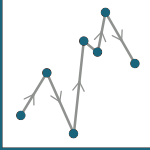
\includegraphics{part1/images/corellation3.png}\\
\textbf{Connected scatterplot:} Usually used to show how the
relationship between 2 variables has changed over time.


\includegraphics{part1/images/corellation4.png}\\
\textbf{Bubble:} Like a scatterplot, but adds additional detail by
sizing the circles according to a third variable.


\includegraphics{part1/images/corellation5.png}\\
\textbf{XY heatmap:} A good way of showing the patterns between 2
categories of data, less effective at showing fine differences in
amounts.

\hypertarget{ranking}{%
\subsubsection{Ranking}\label{ranking}}

Use where an item's position in an ordered list is more important than
its absolute or relative value. Don't be afraid to highlight the points
of interest.

\textbf{Examples:} Comparing indicators of need. Comparing displacement
population figures across sites or districts.


\includegraphics{part1/images/ranking1.png}\\
\textbf{Histogram:} Standard bar charts display the ranks of values much
more easily when sorted into order..


\includegraphics{part1/images/ranking2.png}\\
\textbf{Ordered column:} Same as above but more suited to categories of
dates or with short labels.


\includegraphics{part1/images/ranking3.png}\\
\textbf{Ordered proportional symbol:} Use when there are big variations
between values and/or seeing tne differences between data is not so
important..


\includegraphics{part1/images/ranking4.png}\\
\textbf{Slope:} Perfect for showing how ranks have changed over time or
vary betweencategories.

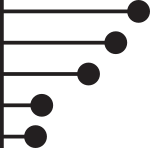
\includegraphics{part1/images/ranking5.png}\\
\textbf{Lollipop:} Lollipops draw more attention to the data value than
standard bar/column and can also show rank and value ef effectively.

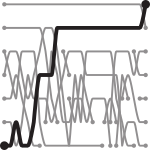
\includegraphics{part1/images/ranking6.png}\\
\textbf{Bump:} Effective for showing changing rankings across multiple
dates. For large datasets,consider grouping lines using colour.

\hypertarget{distribution}{%
\subsubsection{Distribution}\label{distribution}}

Show values in a dataset and how often they occur. The shape (or `skew')
of a distribution can be a memorable way of highlighting the lack of
uniformity or equality in the data.

\textbf{Examples:}

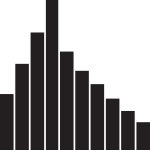
\includegraphics{part1/images/distribution1.png}\\
\textbf{Histogram:} The standard way to show a statistical distribution
- keep the gaps between columns small to highlight the `shape' of the
data.

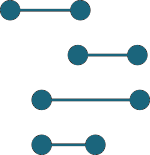
\includegraphics{part1/images/distribution2.png}\\
\textbf{Dot plot:} A simple way of showing the change or range (min/max)
of data across multiple categories.

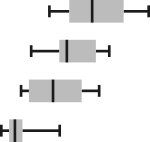
\includegraphics{part1/images/distribution3.png}\\
\textbf{Box plot:} Summarise multiple distributions by showing the
median (centre) and range of the data.


\includegraphics{part1/images/distribution4.png}\\
\textbf{Population pyramid:} A standard way for showing the age and sex
breakdown of a population distribution; effectively, back to back
histograms.


\includegraphics{part1/images/distribution5.png}\\
\textbf{Beeswarm:} Use to emphasise individual points in a distribution.
Points can be sized to an additional variable. Best with medium sized
datasets.

\hypertarget{change-over-time}{%
\subsubsection{Change over time}\label{change-over-time}}

Give emphasis to changing trends. These can be short (intra-day)
movements or extended series traversing decades or centuries: Choosing
the correct time period is important to provide suitable context for the
reader.

\textbf{Examples:}

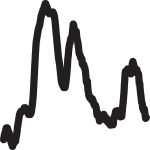
\includegraphics{part1/images/changeovertime1.png}\\
\textbf{Line:} The standard way to show a changing time series. If data
are irregular, consider markers to represent data points.


\includegraphics{part1/images/changeovertime2.png}\\
\textbf{Column:} Columns work well for showing change over time - but
usually best with only one series of data at a time.

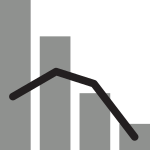
\includegraphics{part1/images/changeovertime3.png}\\
\textbf{Column and timeline:} A good way of showing the relationship
over time between an amount (columns) and a rate (line).


\includegraphics{part1/images/changeovertime4.png}\\
\textbf{Slope:} Good for showing changing data as long as the data can
be simplifed into 2 or 3 points without missing a key part of story.


\includegraphics{part1/images/changeovertime5.png}\\
\textbf{Area chart:} Use with care -- these are good at showingchanges
to total, but seeing change in components can be very difficult.

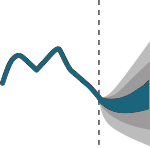
\includegraphics{part1/images/changeovertime6.png}\\
\textbf{Fan chart (projections):} Use to show the uncertainty in future
projections - usually this grows the further forward to projection.

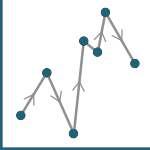
\includegraphics{part1/images/changeovertime7.png}\\
\textbf{Connected scatterplot:} A good way of showing changing data for
two variables whenever there is a relatively clear pattern of
progression.

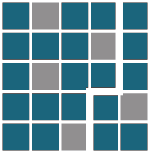
\includegraphics{part1/images/changeovertime8.png}\\
\textbf{Calendar heatmap:} A great way of showing temporal patterns
(daily, weekly, monthly) -- at the expense of showing precision in
quantity.


\includegraphics{part1/images/changeovertime9.png}\\
\textbf{Priestley timeline:} Great when date and duration are key
elements of the story in the data.

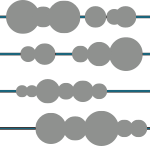
\includegraphics{part1/images/changeovertime10.png}\\
\textbf{Circle timeline:} Good for showing discrete values of varying
size across multiple categories (eg earthquakes by continent).


\includegraphics{part1/images/changeovertime11.png}\\
\textbf{Streamgraph:} A type of area chart; use when seeing changes in
proportions over time is more important than individual values.

\hypertarget{magnitude}{%
\subsubsection{Magnitude}\label{magnitude}}

Show size comparisons. These can be relative (just being able to see
larger/bigger) or absolute (need to see fine differences). Usually these
show a `counted' number (for example, barrels, dollars or people) rather
than a calculated rate or per cent.

\textbf{Examples:}

\includegraphics{part1/images/changeovertime11.png}\\
\textbf{Streamgraph:} A type of area chart; use when seeing changes in
proportions over time is more important than individual values.

\includegraphics{part1/images/magnitude1.png}\\
\textbf{Bar:} See above. Good when the data are not time series and
labels have long category names.

\includegraphics{part1/images/magnitude2.png}\\
\textbf{Paired column:} As per standard column but allows for multiple
series. Can become tricky to read with more than 2 series.

\includegraphics{part1/images/magnitude3.png}\\
\textbf{Marimekko:} A good way of showing the size and proportion of
data at the same time -- as long as the data are not too complicated.

\includegraphics{part1/images/magnitude4.png}\\
\textbf{Isotype (pictogram):} Excellent solution in some instances --
use only with whole numbers (do not slice of an arm to represent a
decimal).

\includegraphics{part1/images/magnitude5.png}\\
\textbf{Radar:}A space-efficient way of showing value of multiple
variables-- but make sure they are organised in a way that makes sense
to reader.

\includegraphics{part1/images/magnitude6.png}\\
\textbf{Parallel coordinates:} A type of area chart; use when seeing
changes in proportions over time is more important than individual
values.

\includegraphics{part1/images/magnitude7.png}\\
\textbf{Grouped symbol:} An alternative to bar/column charts when being
able to count data or highlight individual elements is useful.

\hypertarget{part-to-whole}{%
\subsubsection{Part-to-whole}\label{part-to-whole}}

Show how a single entity can be broken down into its component elements.
If the reader's interest is solely in the size of the components,
consider a magnitude-type chart instead.

\textbf{Examples:}

\includegraphics{part1/images/parttowhole1.png}\\
\textbf{Stacked column or bar:} A simple way of showing part-to-whole
relationships but can be difficult to read with more than a few
components.

\includegraphics{part1/images/parttowhole2.png}\\
\textbf{Radar:}Similar to a pie chart -- but the centre can be a good
way of making space to include more information bout the data (eg
total).

\includegraphics{part1/images/parttowhole3.png}\\
\textbf{Treemap:}Use for hierarchical part-to-whole relationships; can
be difficult to read when there are many small segments.

\includegraphics{part1/images/parttowhole4.png}\\
\textbf{Gridplot:}Good for showing \% information, they work best when
used on whole numbers and work well in small multiple layout form.

\includegraphics{part1/images/parttowhole5.png}\\
\textbf{Venn:}Generally only used for schematic representation.

\includegraphics{part1/images/parttowhole6.png}\\
\textbf{Waterfall:}Can be useful for showing part-to-whole relationships
where some of the components are negative.

\hypertarget{spatial}{%
\subsubsection{Spatial}\label{spatial}}

Aside from locator maps only used when precise locations or geographical
patterns in data are more important to the reader than anything else.

\textbf{Examples:}

\includegraphics{part1/images/spatial1.png}\\
\textbf{Basic choropleth:}The standard approach for putting data on a
map -- should always be rates rather than totals and use a sensible base
geography.

\includegraphics{part1/images/spatial2.png}\\
\textbf{Proportional symbol:} Use for totals rather than rates -- be
wary that small differences in data will be hard to see.

\includegraphics{part1/images/spatial3.png}\\
\textbf{Flowmap:}For showing unambiguous movement across a map.

\includegraphics{part1/images/spatial4.png}\\
\textbf{Contour map:} For showing areas of equal value on a map. Can use
deviation colour schemes for showing +/- values

\includegraphics{part1/images/spatial5.png}\\
\textbf{Dot density:} Used to show the location of individual
events/locations -- make sure to annotate any patterns the reader should
see.

\includegraphics{part1/images/spatial6.png}\\
\textbf{Heatmap:}Can be useful for showing part-to-whole relationships
where some of the components are negative.

\hypertarget{flow}{%
\subsubsection{Flow}\label{flow}}

Show the reader volumes or intensity of movement between two or more
states or conditions. These might be logical sequences or geographical
locations.

\textbf{Examples:}

\includegraphics{part1/images/flow1.png}\\
\textbf{Sankey:}Can be useful for showing part-to-whole relationships
where some of the components are negative.

\includegraphics{part1/images/flow2.png}\\
\textbf{Waterfall:}Can be useful for showing part-to-whole relationships
where some of the components are negative.

\includegraphics{part1/images/flow3.png}\\
\textbf{Network:}Can be useful for showing part-to-whole relationships
where some of the components are negative.

\hypertarget{visual-design-principles}{%
\subsection{Visual Design Principles}\label{visual-design-principles}}

Developed by German psychologists, the Gestalt laws describe how we
interpret the complex world around us. They explain why a series of
flashing lights appear to be moving. And why we read a sentence like
this, \emph{notli ket his ort hat}. Understanding these ``laws'' can be
useful in making sure your message is being conveyed effectively.

\hypertarget{law-of-similarity}{%
\subsubsection{Law of Similarity}\label{law-of-similarity}}

\includegraphics{part1/images/lawofsimilarity.png}\\
The human eye tends to perceive similar elements in a design as a
complete picture, shape, or group, even if those elements are separated.
Examples of this could be the use of symbols to signify conflict on a
map or the use of colour in dots in a scatter plot that are of the same
category.

\hypertarget{law-of-pruxe4gnanz}{%
\subsubsection{Law of Prägnanz}\label{law-of-pruxe4gnanz}}

\includegraphics{part1/images/lawofpragnanz.png}\\
People will perceive and interpret ambiguous or complex images as the
simplest form possible, because it is the interpretation that requires
the least cognitive effort of us. Charts should aim to be as complex as
necessary and as simple as possible to convey their meaning.
\href{https://en.wikipedia.org/wiki/Edward_Tufte}{Edward Tufte} calls
this the data-ink ratio.

\hypertarget{law-of-proximity}{%
\subsubsection{Law of Proximity}\label{law-of-proximity}}

\includegraphics{part1/images/lawofproximity.png}\\
Objects that are near, or proximate to each other, tend to be grouped
together.\\
An example of this could be a grouped bar chart where for the funding
for each year is grouped by donor.

\hypertarget{law-of-continuity}{%
\subsubsection{Law of Continuity}\label{law-of-continuity}}

\includegraphics{part1/images/lawofcontinuity.png}\\
Elements that are visually connected are perceived as more related than
elements with no connection. This principle is visible when using a line
graph to connect point values.

\hypertarget{law-of-common-region}{%
\subsubsection{Law of Common Region}\label{law-of-common-region}}

\includegraphics{part1/images/lawofcommonregion.png}\\
Elements tend to be perceived into groups if they are sharing an area
with a clearly defined boundary. This law is perhaps most commonly used
in maps, where administrative boundaries are shown with solid or dashed
lines.

When presenting static charts a useful tip is to use
\href{https://en.wikipedia.org/wiki/Annotation}{annotation} to guide the
viewer through the graph, to put the data in context and to highlight
the key relevant facts. \footnote{Data journalism put increasing
  emphasis on the need for a good annotation layer, as can be seen by
  this article from the
  \href{https://www.ft.com/content/4743ce96-e4bf-11e7-97e2-916d4fbac0da}{Financial
  Times}}

\hypertarget{use-of-colour}{%
\subsection{Use of Colour}\label{use-of-colour}}

When choosing colours in your charts its important to understand
possible local significance that may be associated to a specific colour.
For instance, in one country a colour may signify good luck, whereas in
a different country, the same colour could be associated with a
non-state armed group.\footnote{ACAPS have a great guide on the
  \href{https://www.acaps.org/use-colour-data-display}{Use of Colour in
  Data Display}}

Where possible, special attention should be taken to ensure that chart
remain readable when printed in gray scale and that they are colour
blind safe, meaning that the chart should not be confusing for people
with red-green colour blindness (an estimated 8\% of men and 0.4\% of
women).

Adding to the previous description of the role of color in perception,
the use of colour in scales, particularly maps, typically takes one of
the following three forms.\footnote{More details on
  \href{https://www.humanitarianresponse.info/en/programme-cycle/space}{HumanitarianResponse.info}}

\begin{enumerate}
\def\labelenumi{\arabic{enumi}.}
\item
  \includegraphics{part1/images/sequential-scale.png}
  \textbf{Continuous(sequential) scales} used to show values going from
  low to high. Eg. population density per district.
\item
  \includegraphics{part1/images/diverging-scale.png} \textbf{Diverging
  scales} which visualize difference from a norm, such as
  \href{https://storymaps.arcgis.com/stories/a371cdf9462b4dca9051b9f60a3185bc}{this
  example} showing location in St Vincent that showed both net inward
  and outward movements of people following the eruption of a volcano.
\item
  \includegraphics{part1/images/qualitative-scale.png}\textbf{Categorical(qualitative)
  scales} used to distinguish different (non numeric) objects eg. a map
  using different shades for different countries.
\end{enumerate}

Two of the most common ways to respresent colour are RGB and CMYK. RGB,
commonly used on websites can be shown as a hex number or RGB number.
For printed materials where colour accuracy is important, CYMK is
typically used. Not all software supports the CMYK colour space, so if
color accuracy is important you may want to use an Adobe tool such as
Illustrator or In Design to apply finishing touches to print
materials.\footnote{For a detailed explanation of RGB and CMYK and how
  they differ, see
  \href{https://en.99designs.ch/blog/tips/correct-file-formats-rgb-and-cmyk/}{here}}

\hypertarget{presenting}{%
\section{Presenting}\label{presenting}}

Having a great data collection system, doing great analysis and creating
effective visuals don't necessarily lead to informing or changing
decision by themselves. An important skill for IMOs that is often
overlooked is the importance of verbal communication and presentation
skills, be in in an in-person context such as a Cluster meeting or as is
becoming more common, web-based calls. These meeting offer an important
window of opportunity where, if communicated clearly and in a convincing
manner a good analysis can meet it's objectives.

The following video is an example of effective communication, where the
speaker shows a clear understanding of his audience(s), succinctly
describes the context, the cause, the call for action (giving specific
examples) and the urgency and scale.

When presenting slides, consider the following:

\begin{itemize}
\item
  \textbf{Only one idea per slide} Having multiple ideas presented will
  distract your audience and confuse your key message.
\item
  \textbf{Explain your point, then show slide.} Your audience can
  interpret either the visuals on screen or your spoken message. It is
  very difficult to both at the same time.
\item
  \textbf{Speaker is the star, not the slides.} The slides exist to aide
  the communication of the speaker, not to distract from it.
\item
  \textbf{Never read from the slides.} It portrays a lack of
  preparedness and dilutes the communication rather than complimenting
  it.
\item
  \textbf{Keep your hands free to move.} Not verbal expression can help
  the audience relate to the message and can help emphasise key
  messages.
\item
  \textbf{Tell a story to drive home your message} Conveying your
  message through a narrative is a powerful way to introduce your
  audience with your key points, for them to engage with the topic and
  to remember it.
\item
  \textbf{Use photos and drawings on slides.} Photos can help bring an
  emotive human element into otherwise abstract messages. Effective
  visuals can communicate concepts that would be much harder to explain
  through written or spoken word alone.
\item
  \textbf{Face your audience, not your slides.} You are trying to
  convince, your audience, not the slides.
\item
  \textbf{Avoid complexity.} Unnecessary complexity is a barrier for
  comprehension and can cause your audience to disengage with the topic.
\item
  \textbf{Rehearse, rehearse, rehearse.}
\end{itemize}

\hypertarget{data-responsibility}{%
\chapter{Data Responsibility}\label{data-responsibility}}

This chapter is in draft stage.

This section describes data security; data protection

Here's my note!

\textbf{Outline} - Main resources: IASC Data Responsibility in
Humanitarian Action; ICRC Handbook on Data Protection in Humanitarian
Action; IOM Data Protection Manual - Explain what is personal
information - Examples of types of data in CCCM - Data protection
principles

IASC Data Responsibility in Humanitarian Action

ICRC Handbook on Data Protection in Humanitarian Action

IOM Data Protection Manual

\hypertarget{tools}{%
\chapter{Tools}\label{tools}}

\hypertarget{test}{%
\section{test}\label{test}}

The choice of software used to create CCCM products can be influenced by
factors such as personal preference/familiarity, experience - some IMs
may prefer more advanced tools, time constraints and budget. The
following list of software is not a prescriptive list, rather a list of
tools preferred by the authors

\hypertarget{microsoft-excel}{%
\subsection{Microsoft Excel}\label{microsoft-excel}}

.

\hypertarget{qgisarcgis}{%
\subsection{QGIS/ArcGIS}\label{qgisarcgis}}

.

\hypertarget{inkscapeadobe-illustrator}{%
\subsection{Inkscape/Adobe
Illustrator}\label{inkscapeadobe-illustrator}}

.

\hypertarget{microsoft-powerbi}{%
\subsection{Microsoft PowerBI}\label{microsoft-powerbi}}

.

\hypertarget{microsoft-formsgoogle-forms}{%
\subsection{Microsoft Forms/Google
Forms}\label{microsoft-formsgoogle-forms}}

.

\hypertarget{kobo-toolbox}{%
\subsection{Kobo toolbox}\label{kobo-toolbox}}

.

\hypertarget{advanced-tools}{%
\section{Advanced tools}\label{advanced-tools}}

.

\part{CCCM Operations IM}

\hypertarget{the-role-of-im-in-cccm-operations}{%
\chapter{The role of IM in CCCM
Operations}\label{the-role-of-im-in-cccm-operations}}

This part of the handbook will be drafted following the completion of
the Part 1 -
\href{https://imhandbook.cccmcluster.org/part1/data-literacy.html}{Humanitarian
IM} and Part 3 -
\href{https://imhandbook.cccmcluster.org/part3/cluster.html}{CCCM
Cluster IM} of the handbook

\hypertarget{products-templates}{%
\chapter{Products \& Templates}\label{products-templates}}

\begin{tcolorbox}[enhanced jigsaw, colframe=quarto-callout-warning-color-frame, title=\textcolor{quarto-callout-warning-color}{\faExclamationTriangle}\hspace{0.5em}{Warning}, toptitle=1mm, toprule=.15mm, colbacktitle=quarto-callout-warning-color!10!white, breakable, arc=.35mm, coltitle=black, bottomrule=.15mm, titlerule=0mm, opacityback=0, rightrule=.15mm, bottomtitle=1mm, leftrule=.75mm, left=2mm, opacitybacktitle=0.6, colback=white]

Drafting of this chapter has not yet started.

\end{tcolorbox}

note: For some products, the operating environment may dictate wherether
certain tools are designed at the CCCM partner level or at the Cluster
level. For example, in some countries, the CCCM Cluster designed and
manages a single system for Complaint and Feedback, whereas in other
contexts each CCCM partner design and manage their own system.

\part{CCCM Cluster IM}

\hypertarget{the-role-of-im-in-the-cluster}{%
\chapter{The role of IM in the
Cluster}\label{the-role-of-im-in-the-cluster}}

\begin{tcolorbox}[enhanced jigsaw, colframe=quarto-callout-warning-color-frame, title=\textcolor{quarto-callout-warning-color}{\faExclamationTriangle}\hspace{0.5em}{Warning}, toptitle=1mm, toprule=.15mm, colbacktitle=quarto-callout-warning-color!10!white, breakable, arc=.35mm, coltitle=black, bottomrule=.15mm, titlerule=0mm, opacityback=0, rightrule=.15mm, bottomtitle=1mm, leftrule=.75mm, left=2mm, opacitybacktitle=0.6, colback=white]

Part 3 of the IM handbook is in a zero draft phase. Both the structure
and content are likley to change significantly

\end{tcolorbox}

\begin{tcolorbox}[enhanced jigsaw, colframe=quarto-callout-tip-color-frame, title=\textcolor{quarto-callout-tip-color}{\faLightbulb}\hspace{0.5em}{Recommended reading}, toptitle=1mm, toprule=.15mm, colbacktitle=quarto-callout-tip-color!10!white, breakable, arc=.35mm, coltitle=black, bottomrule=.15mm, titlerule=0mm, opacityback=0, rightrule=.15mm, bottomtitle=1mm, leftrule=.75mm, left=2mm, opacitybacktitle=0.6, colback=white]

\begin{itemize}
\tightlist
\item
  \href{files/humanitarianprofilesupportguidance_final_may2016.pdf}{Humanitarian
  Population Figures} - IMWG
\item
  \href{files/humanitarianprofilesupportguidance_final_may2016.pdf}{IASC
  Reference Module for the Implementation of the Humanitarian Programme
  Cycle}- IASC
\item
  \href{files/Operational\%20Guidance\%20on\%20Responsibilities\%20of\%20Cluster-Sector\%20Leads\%20and\%20OCHA\%20in\%20Information\%20Management.pdf}{Responsibilities
  of Cluster/Sector Leads and OCHA in Information Management} - IASC
  (2008)
\end{itemize}

\end{tcolorbox}

The role of Information Management in the CCCM Cluster at country-level
is best viewed through the lens of the \textbf{six core
functions}:\footnote{From the
  \href{files/Reference\%20Module\%20for\%20Cluster\%20Coordination\%20at\%20Country\%20Level.pdf}{IASC
  Reference Module for Cluster Coordination at Country Level, revised
  July 2015}}

\begin{quote}
\begin{enumerate}
\def\labelenumi{\arabic{enumi}.}
\tightlist
\item
  To support service delivery by:

  \begin{itemize}
  \tightlist
  \item
    Providing a platform that ensures service delivery is driven by the
    Humanitarian Response Plan and strategic priorities.
  \item
    Developing mechanisms to eliminate duplication of service delivery.
  \end{itemize}
\end{enumerate}
\end{quote}

The IM role supports service delivery by ensuring information systems
are in place to understand where CCCM partners and activities are
conducted, where there are gaps or overlaps and how those activities are
meeting the overall objectives and targets decided upon by the cluster.

\begin{quote}
\begin{enumerate}
\def\labelenumi{\arabic{enumi}.}
\setcounter{enumi}{1}
\tightlist
\item
  To inform the HC/HCT's strategic decision-making by:

  \begin{itemize}
  \tightlist
  \item
    Preparing needs assessments and analysis of gaps (across and within
    clusters, using information management tools as needed) to inform
    the setting of priorities.
  \item
    Identifying and finding solutions for (emerging) gaps,
    obstacles,duplication and cross-cutting issues.
  \item
    Formulating priorities on the basis of analysis.
  \end{itemize}
\end{enumerate}
\end{quote}

By collecting and analysing CCCM needs to inform; an understanding of
gaps; barriers for the response; where and whom requires prioritization.

\begin{quote}
\begin{enumerate}
\def\labelenumi{\arabic{enumi}.}
\setcounter{enumi}{2}
\tightlist
\item
  To plan and implement cluster strategies by:

  \begin{itemize}
  \tightlist
  \item
    Developing sectoral plans, objectives and indicators that directly
    support realization of the overall response's strategic objectives.
  \item
    Applying and adhering to common standards and guidelines.
  \item
    Clarifying funding requirements, helping to set priorities, and
    agreeing cluster contributions to the HC's overall humanitarian
    funding proposals.
  \end{itemize}
\end{enumerate}
\end{quote}

To support the setting of measurable objectives and indicators, the
categorization of activities and cost estimations for these activities
or projects.

\begin{quote}
\begin{enumerate}
\def\labelenumi{\arabic{enumi}.}
\setcounter{enumi}{3}
\tightlist
\item
  To monitor and evaluate performance by:

  \begin{itemize}
  \tightlist
  \item
    Monitoring and reporting on activities and needs.
  \item
    Measuring progress against the cluster strategy and agreed results.
  \item
    Recommending corrective action where necessary.
  \end{itemize}
\end{enumerate}
\end{quote}

To manage systems that monitor collective progress against the set
targets and objected.

\begin{quote}
\begin{enumerate}
\def\labelenumi{\arabic{enumi}.}
\setcounter{enumi}{4}
\tightlist
\item
  To build national capacity in preparedness and contingency planning.
\end{enumerate}
\end{quote}

To disseminate the above skills, systems and processes to national and
local levels to ensure national-level preparedness on systems and skills
relevant to CCCM.

\begin{quote}
\begin{enumerate}
\def\labelenumi{\arabic{enumi}.}
\setcounter{enumi}{5}
\tightlist
\item
  To support robust advocacy by:

  \begin{itemize}
  \tightlist
  \item
    Identifying concerns, and contributing key information and messages
    to HC and HCT messaging and action.
  \item
    Undertaking advocacy on behalf of the cluster, cluster members, and
    affected people.
  \end{itemize}
\end{enumerate}
\end{quote}

Evidence-based advocacy, to inform strategic decision making and to
represent the challenges, needs and achievements of the cluster.

\hypertarget{the-humanitarian-program-cycle}{%
\section{The Humanitarian Program
Cycle}\label{the-humanitarian-program-cycle}}

\includegraphics{part3/images/HPCcycle.png}

\begin{quote}
The humanitarian programme cycle (HPC) is a coordinated series of
actions undertaken to help prepare for, manage and deliver humanitarian
response. It consists of five elements coordinated in a seamless manner,
with one step logically building on the previous and leading to the
next. Successful implementation of the humanitarian programme cycle is
dependent on effective emergency preparedness, effective coordination
with national/local authorities and humanitarian actors, and information
management. \footnote{More details on
  \href{https://www.humanitarianresponse.info/en/programme-cycle/space}{HumanitarianResponse.info}}
\end{quote}

\hypertarget{needs-assessment-analysis}{%
\chapter{Needs Assessment \& Analysis}\label{needs-assessment-analysis}}

\begin{tcolorbox}[enhanced jigsaw, colframe=quarto-callout-tip-color-frame, title=\textcolor{quarto-callout-tip-color}{\faLightbulb}\hspace{0.5em}{Recommended reading}, toptitle=1mm, toprule=.15mm, colbacktitle=quarto-callout-tip-color!10!white, breakable, arc=.35mm, coltitle=black, bottomrule=.15mm, titlerule=0mm, opacityback=0, rightrule=.15mm, bottomtitle=1mm, leftrule=.75mm, left=2mm, opacitybacktitle=0.6, colback=white]

\begin{itemize}
\tightlist
\item
  \href{files/humanitarian_needs_assessment-the_good_enough_guide_2014.pdf}{Humanitarian
  Needs Assessment: The Good Enough Guide} - ACAPS
\item
  \href{files/4.\%20HPC_2023-JIAF_Guide\%201.1.pdf}{JIAF 1.1 Guidance}
\end{itemize}

\end{tcolorbox}

\hypertarget{cccm-sectoral-analysis}{%
\section{CCCM Sectoral analysis}\label{cccm-sectoral-analysis}}

a

\hypertarget{setting-your-needs-analysis-parameters}{%
\subsection{Setting your needs analysis
parameters}\label{setting-your-needs-analysis-parameters}}

a

\hypertarget{people-in-need-calculation}{%
\subsection{People in Need
calculation}\label{people-in-need-calculation}}

a

\hypertarget{severity-of-needs-in-cccm}{%
\subsection{Severity of needs in CCCM}\label{severity-of-needs-in-cccm}}

a

\hypertarget{inter-sectoral-analysis}{%
\section{Inter-sectoral analysis}\label{inter-sectoral-analysis}}

a

\hypertarget{humanitarian-needs-overview-flash-appeals}{%
\section{Humanitarian Needs Overview \& Flash
Appeals}\label{humanitarian-needs-overview-flash-appeals}}

a

\hypertarget{strategic-planning}{%
\chapter{Strategic Planning}\label{strategic-planning}}

\hypertarget{strategic-objectives}{%
\section{Strategic Objectives}\label{strategic-objectives}}

.

\hypertarget{indicators-1}{%
\section{Indicators}\label{indicators-1}}

.

\hypertarget{activities-1}{%
\section{Activities}\label{activities-1}}

.

\hypertarget{targets}{%
\section{Targets}\label{targets}}

\hypertarget{humanitarian-response-plan}{%
\section{Humanitarian Response Plan}\label{humanitarian-response-plan}}

.

\hypertarget{resource-mobilization}{%
\chapter{Resource Mobilization}\label{resource-mobilization}}

\hypertarget{costing}{%
\section{Costing}\label{costing}}

.

\hypertarget{implementation-monitoring}{%
\chapter{Implementation \& Monitoring}\label{implementation-monitoring}}

\begin{tcolorbox}[enhanced jigsaw, colframe=quarto-callout-tip-color-frame, title=\textcolor{quarto-callout-tip-color}{\faLightbulb}\hspace{0.5em}{Recommended reading}, toptitle=1mm, toprule=.15mm, colbacktitle=quarto-callout-tip-color!10!white, breakable, arc=.35mm, coltitle=black, bottomrule=.15mm, titlerule=0mm, opacityback=0, rightrule=.15mm, bottomtitle=1mm, leftrule=.75mm, left=2mm, opacitybacktitle=0.6, colback=white]

\begin{itemize}
\tightlist
\item
  \href{files/OCHA\%20Approaches\%20to\%20determining\%20people\%20reached\%202022.pdf}{Measuring
  and aggregating population figures for planning and monitoring}
\end{itemize}

\end{tcolorbox}

\hypertarget{people-reached}{%
\section{People Reached}\label{people-reached}}

.

\hypertarget{people-covered}{%
\section{People Covered}\label{people-covered}}

.

\hypertarget{operational-peer-review-evaluation}{%
\chapter{Operational Peer Review \&
Evaluation}\label{operational-peer-review-evaluation}}

\hypertarget{cluster-coordination-performance-monitoring}{%
\section{Cluster Coordination Performance
Monitoring}\label{cluster-coordination-performance-monitoring}}

.


\backmatter

\end{document}
